\documentclass[11pt]{article}
\usepackage{graphicx}  % Include figure files
\usepackage{hyperref}

\begin{document}
%\title{Estimation of SBS experiments event size and disk use}

%\maketitle

\paragraph{Question 3}
{\it Inelastic scattering contribution is discussed, but I'm still a
little confused. You state that this background is small.
Great, but how uncertain is it?}\\
{\it The singles rate in HCal is huge and apparently the coincidence rate between BigBite and HCal is also large. 
How uncertain is the inelastic rate?}\\
{\it You base it on a model, how valid is it for your needs?}\\
{\it How much of the inelastic tail do you measure, e.g. how much of Figs. 10 and 11 will come from data?}
{\it If this background is twice as big as you expect, do you have recourse?}\\

``Inelastic scattering contribution is discussed, but I'm still a little confused. You state that this background is small. Great, but how uncertain is it?''\\

The statement made in our proposal is that the inelastic scattering contribution to the quasi-elastic statistics is low. To be specific, in this context, we are discussing the $e-N$ scattering in the resonance region.
Our quasi-elastic $e-N$ MC generator uses the Kelly form factor fits\footnote{Phys. Rev. C 70, 068202 (2004)}.% to weigh our quasi-elastic events.\\
Our inelastic resonant $e-N$ MC generator uses the model by P.~Bosted and E.~Christy\footnote{Phys.~Rev.~C81.055213, https://arxiv.org/abs/0712.3731}. %See also the GMn E12-09-019 proposal page (attached).
This model is a fit of $e-N$ data in the resonance region from Jefferson Lab Hall C\footnote{http://arxiv.org/abs/nucl-ex/0410027} which covers $0<=Q^2<8 {\rm (GeV/c)}^2$, with beam energies up to 5.5 GeV.
According to $^2$, %\footnote{Phys.~Rev.~C81.055213, https://arxiv.org/abs/0712.3731},
the fit residue to the data between 4 and 6 GeV fluctuates by $\pm$ 10\%. We assume a 20\% systematic uncertainty on our inelastic cross section. %background estimation.

%After the analysis detailed below,
We have determined that the inelastic scattering contribution to our quasi-elastic sample, within the analysis and selection detailed below, is less than 1\%, with 0.2\% uncertainty.


As discussed in the proposal, the relevant variables to select the quasi-elastic $e-N$ scattering from the resonant $e-N$ scattering are the missing mass $W^2 = M_{N}^2+2M_{N}^{2}(E-E')-Q^2$, evaluated with the BigBite resolution, of the system N$(e, e')X$, and the transverse missing momentum.
Figure~\ref{fig:W2} displays the event distributions in $W^2$ for both our simulated quasi-elastic and inelastic samples within the following set of fiducial acceptance cuts:
%
\begin{itemize}
\item{the electron track is reconstructed in BigBite;}
\item{the total energy deposited in the BigBite calorimeter is above the 3 GeV threshold for an average 4.2 GeV elastic peak (for $\epsilon = 0.84$ kinematic);}
\item{the electron track must fire at least 3 PMTs in the GRINCH detectors;}
\item{the total energy deposited in HCal is above the 0.10 GeV threshold. This corresponds to 90\% efficiency of the 3.2 GeV/c nucleons which deposit 0.20 GeV in the HCal (scintillator material).}
\end{itemize}
%
%According to $^3$, %\footnote{Phys.~Rev.~C81.055213, https://arxiv.org/abs/0712.3731},
%the fit residue to the data between 4 and 6 GeV fluctuates by $\pm$ 10\%. We assume a 20\% systematic error attached on our inelastic background estimation.% or 0.4\% relative quasi-elastic.\\
%
\begin{figure}[h]
  \centering
    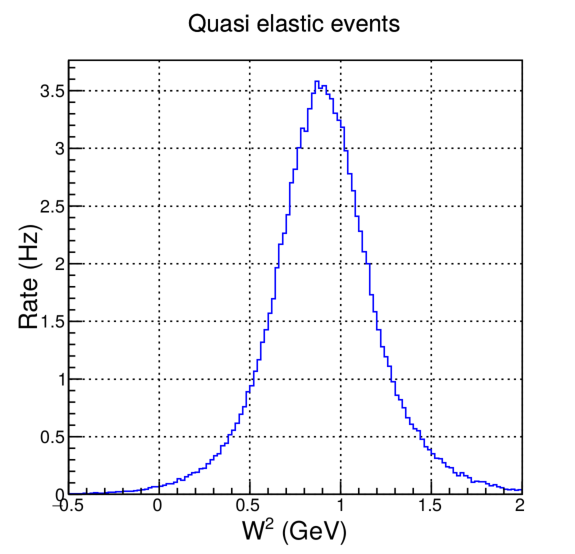
\includegraphics[width=5cm]{W2_sig.pdf}
    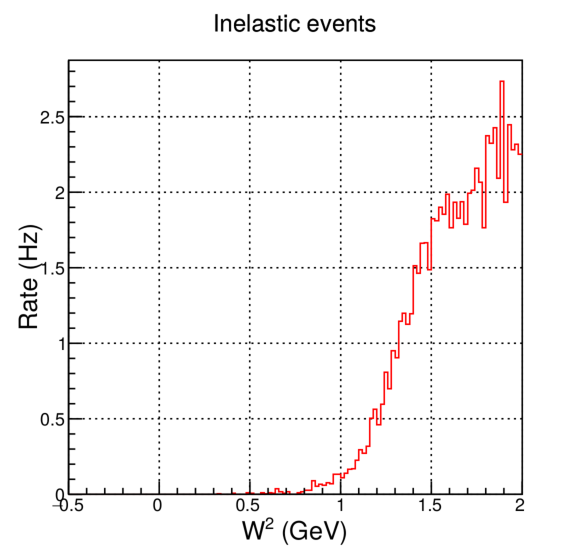
\includegraphics[width=5cm]{W2_inel.pdf}
    \caption{Event distributions in $W^2 = M_{N}^2+2M_{N}^{2}(E-E')-Q^2$  for quasi elastic $e-N$ (left) and inelastic resonant $e-N$ (right) within the fiducial analysis cuts.}
    \label{fig:W2}
\end{figure}
%

Before reconstructing the nucleon momentum, it is necessary to apply a selection cut on $W^2$ to reject a fraction of the inelastic events. To this end, only events for which $W^2<1.10~{\rm GeV}^2$ are selected for further discussion. Within this selection, our total number of events counts 97\% of quasi-elastic and 3\% of inelastic.
% this cut is 76\% for quasi-elastic and 1\% for inelastic.

Now we will discuss the missing perpendicular momentum.
The nucleon momentum and direction is reconstructed using the position of the HCal cluster, on the first step {\em under the assumption that it is a neutron}.
We use the direction of the virtual photon vector $\vec{q}$ (corrected with the vertex position) to project the expected neutron position.
The difference between the reconstructed and the projected nucleon position is shown, projected on $x$ (the non-dispersive direction) and $y$ (the dispersive direction), for both quasi-elastic and inelastic events on figure~\ref{hcal_id_2D}.
%
\begin{figure}[!h]
  \centering
    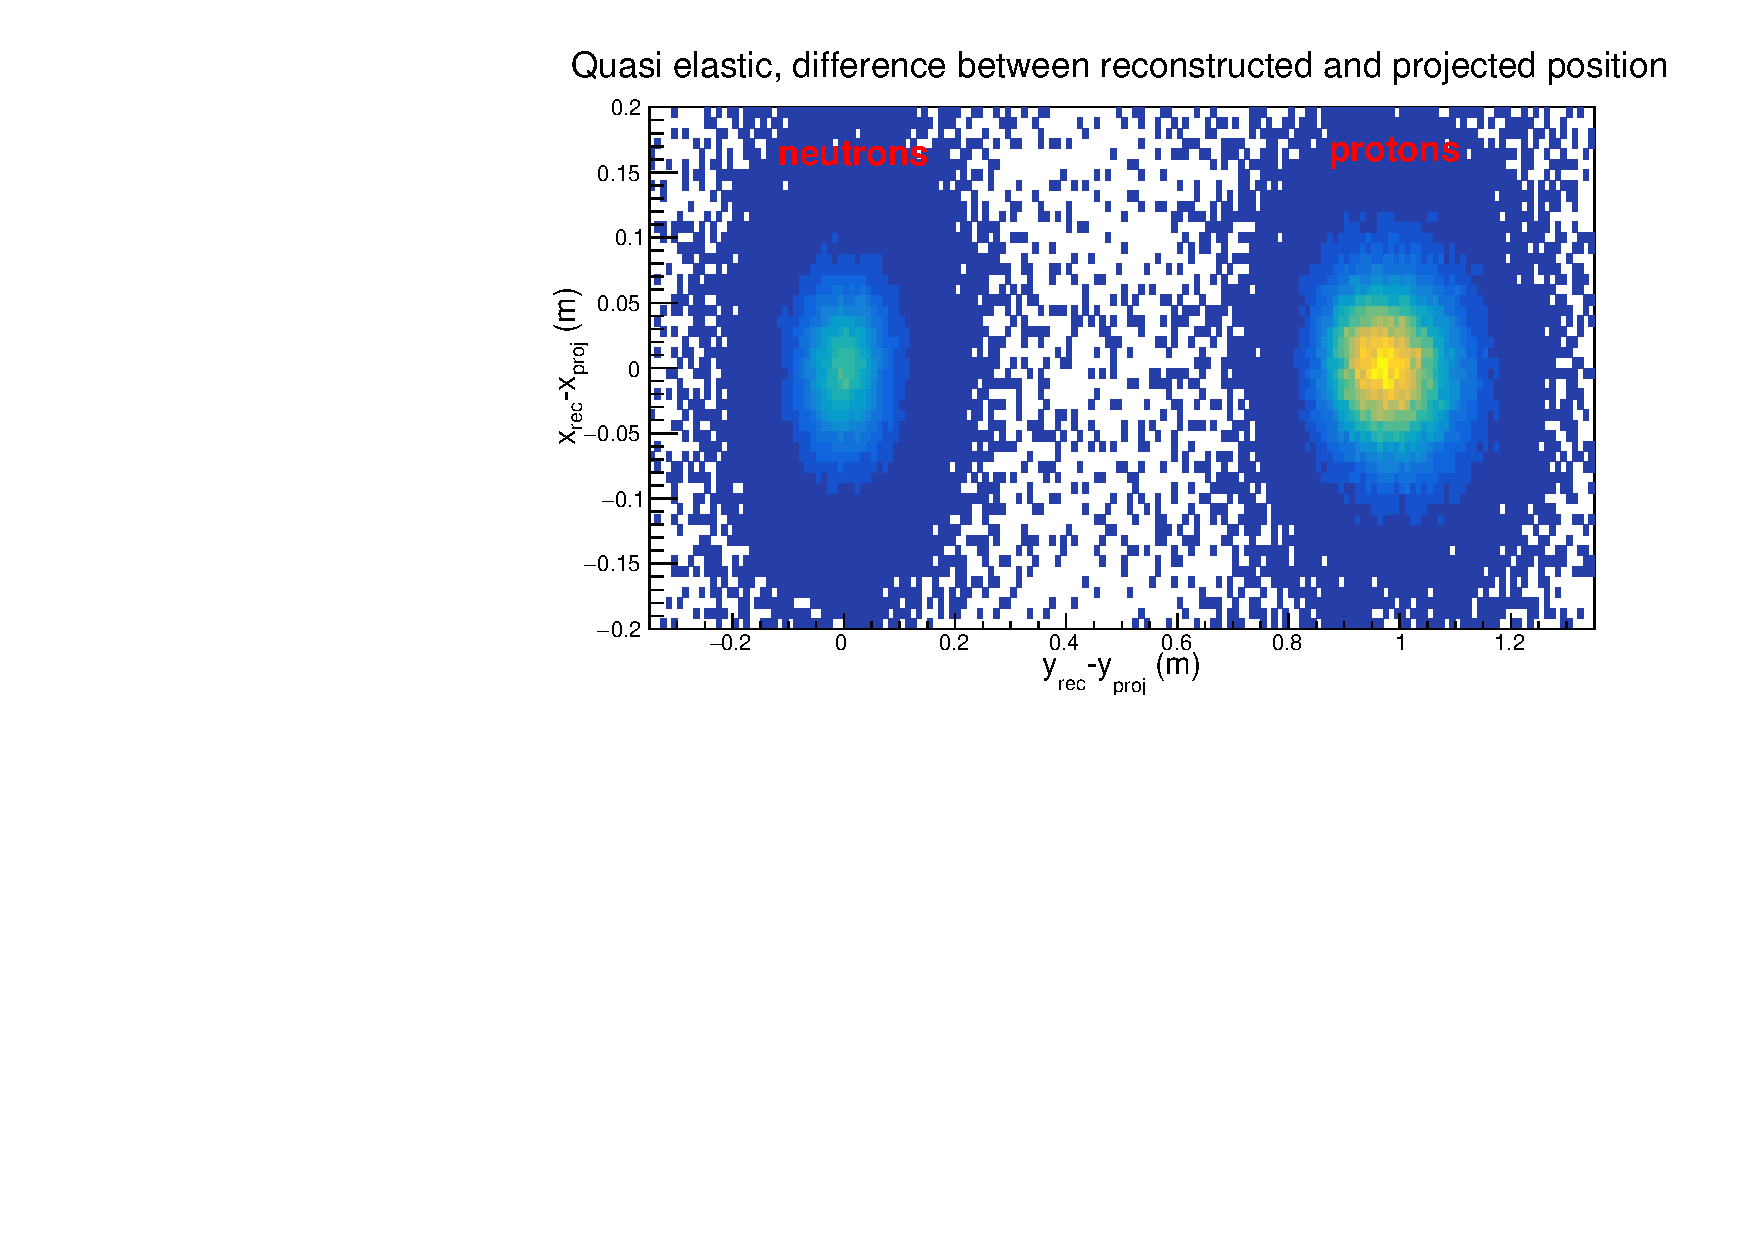
\includegraphics[width=6cm]{HCal_PID_QE.pdf}
    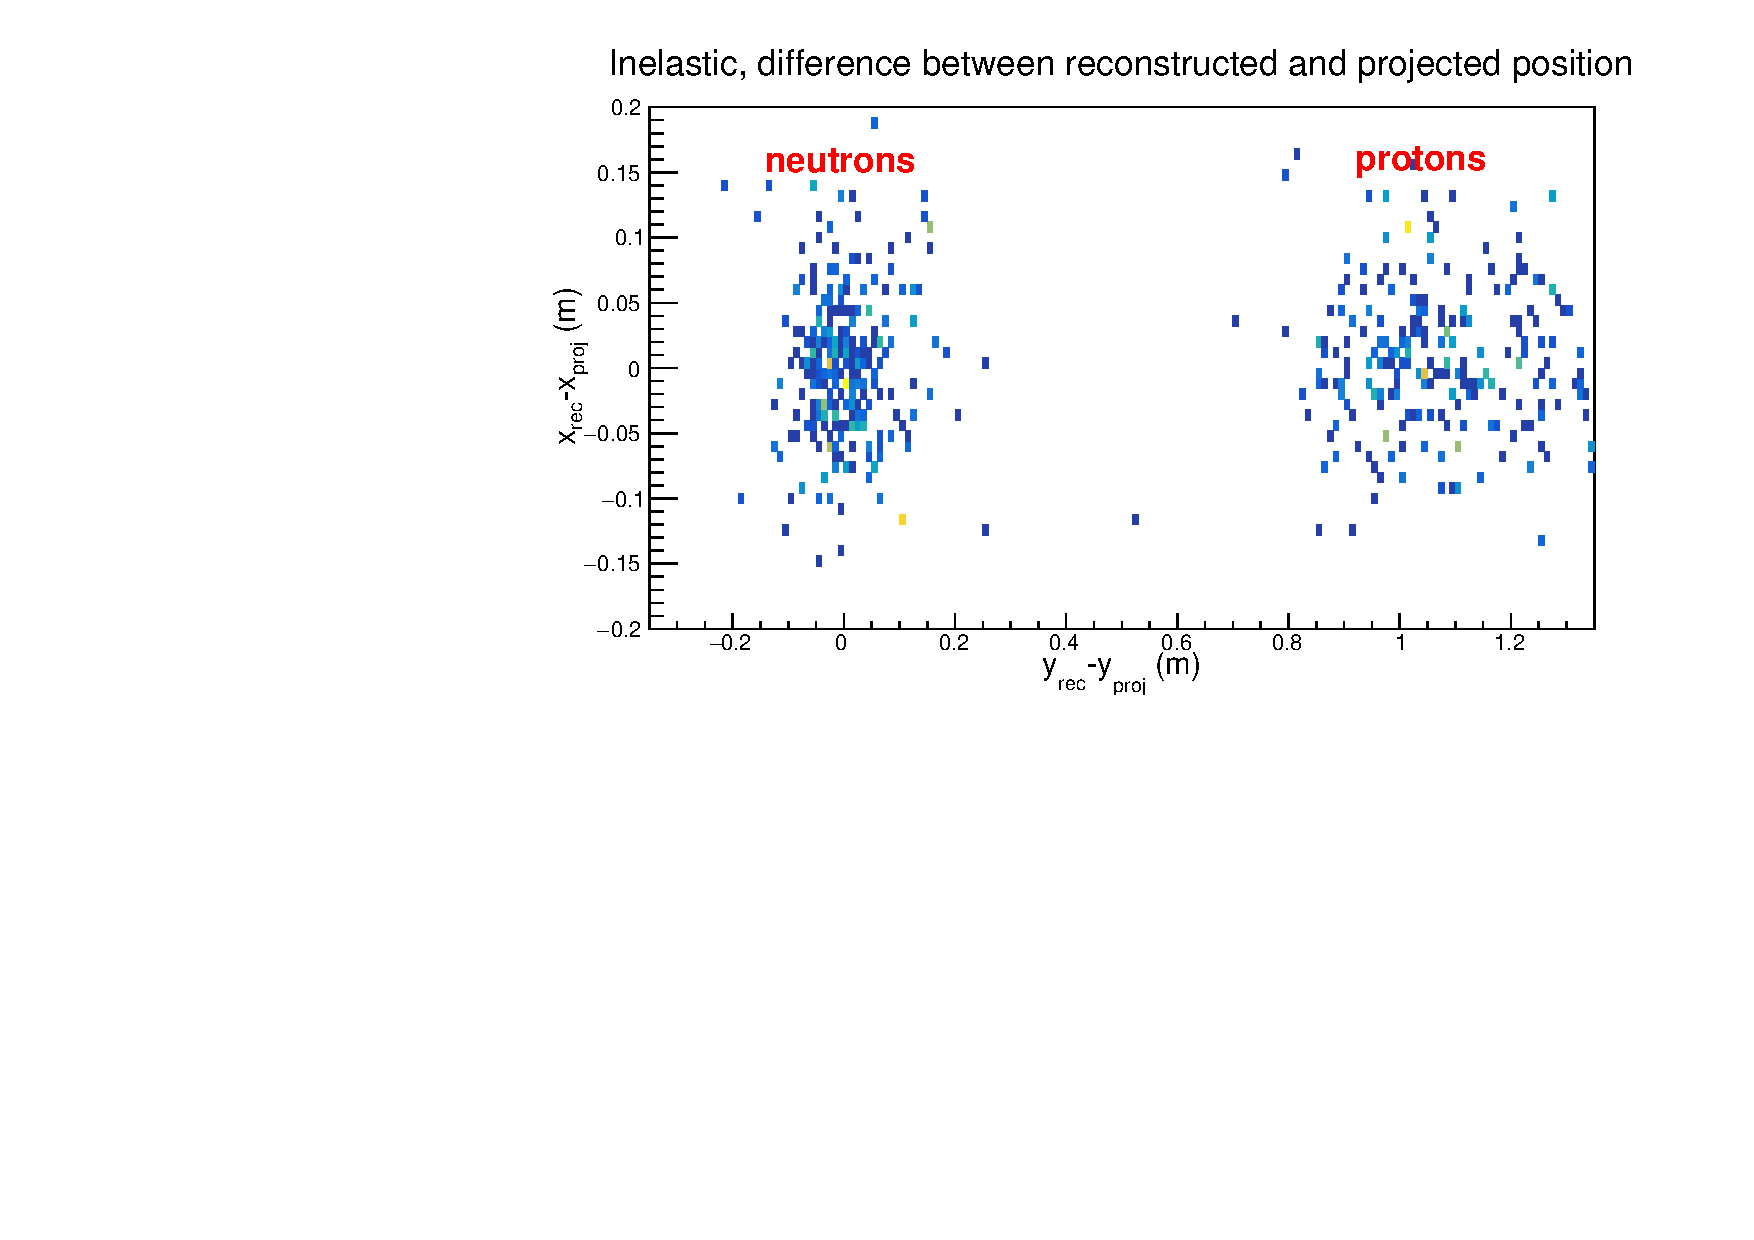
\includegraphics[width=6cm]{HCal_PID_Inel.pdf}
    \caption{Difference of projected position and reconstructed position for the nucleons in $x$ (non-dispersive direction) and $y$ (dispersive direction), for quasi-elastic events (left) and inelastic events (right). On each plot We clearly notice two structures. The structure on the left, centered at 0, is due to the neutrons. The structure on the right, shifted by about 1~m is due to the protons, which are deflected upwards by the magnetic field. 
    }
    \label{hcal_id_2D}
\end{figure}
%
We clearly distinguish in each case two structures, one which can be identified a the neutrons, centered on zero in both $x$ and $y$, and one which can be identified as the protons, which are deflected upwards and are shifted by about 1~m in $y$.
Figure~\ref{hcal_id_y} also shows the difference between the reconstructed and the projected nucleon position, except projected on $y$ (the dispersive direction), for both the quasi-elastic and inelastic events. Comparing both the expected inelastic and elastic yields in this variable side-by-side evidences further the important role of the $W^2<1.10~{\rm GeV}^2$ selection to filter out inelastic events. 
%
\iffalse
\begin{figure}[!h]
  \centering
    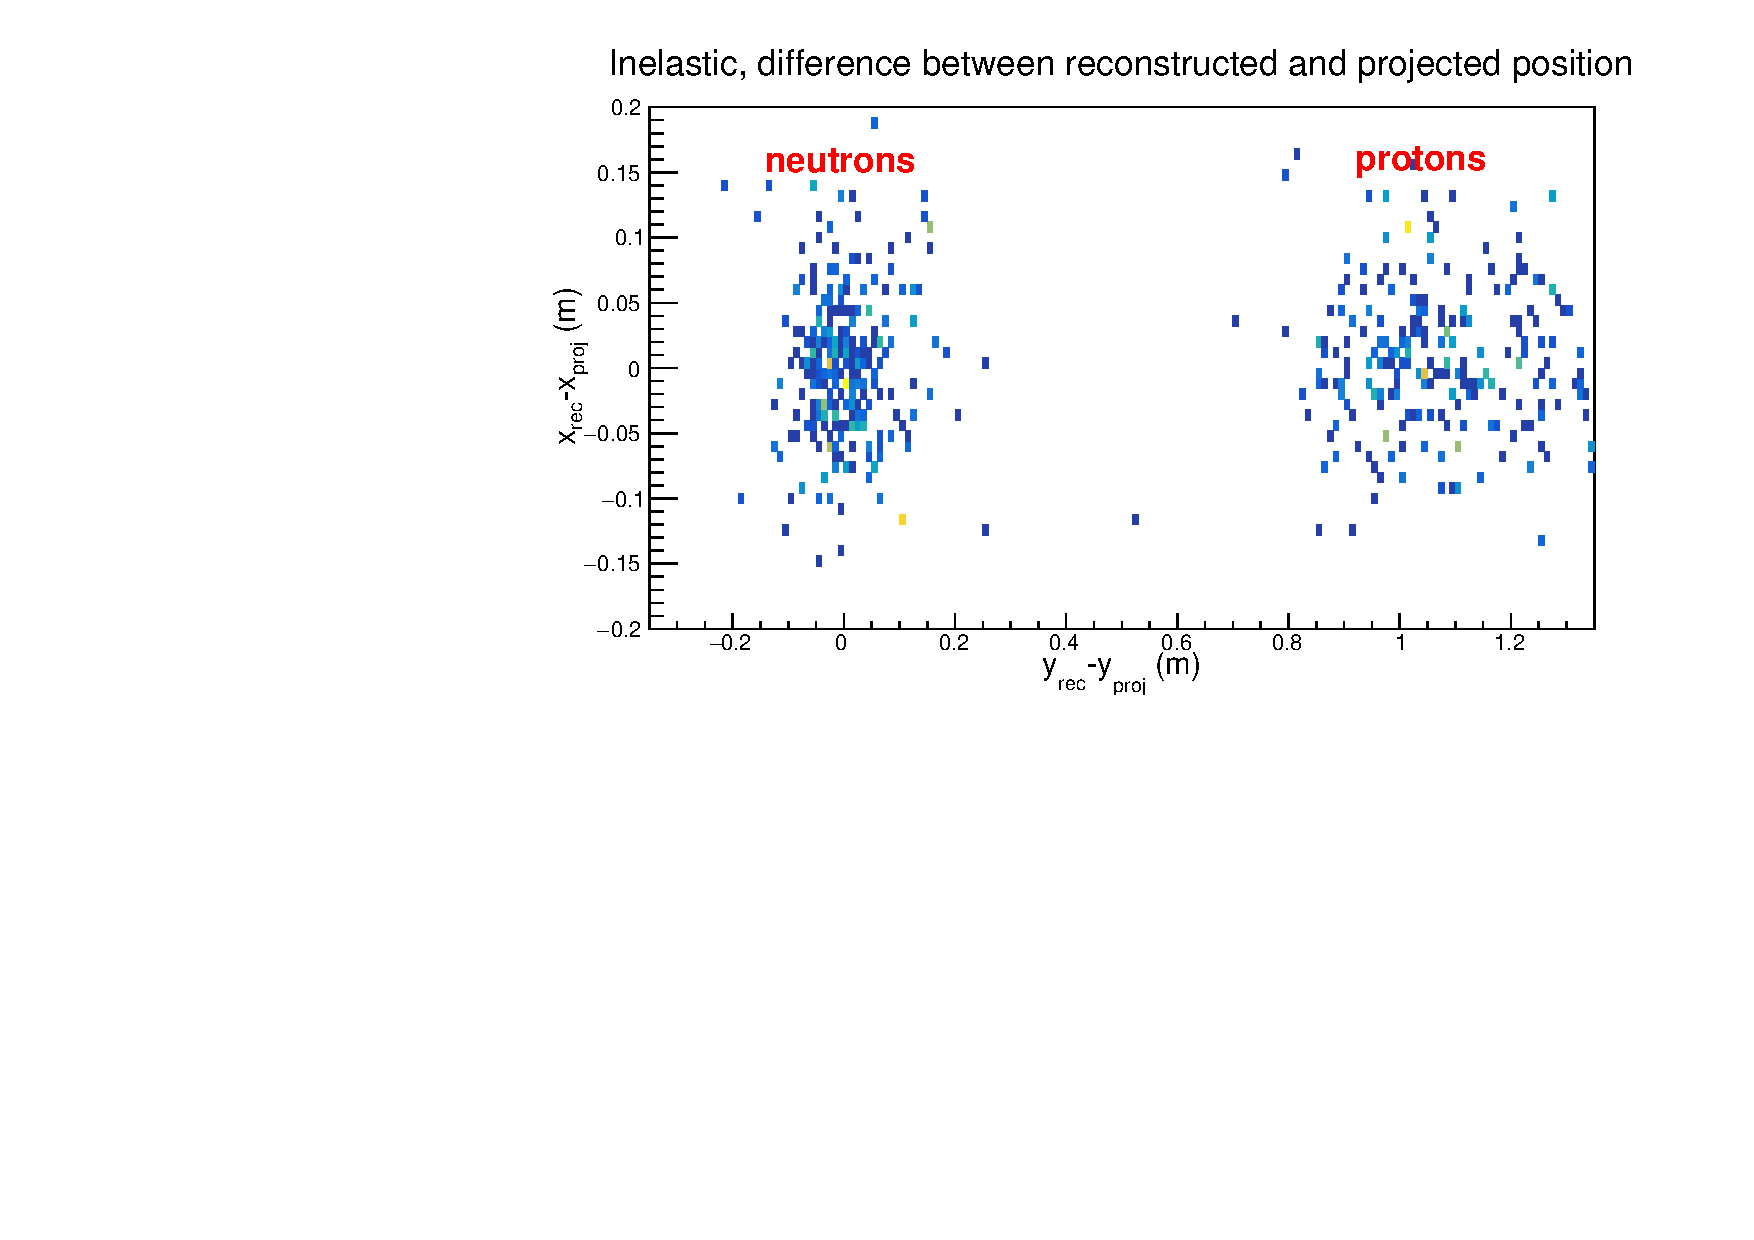
\includegraphics[width=10cm]{HCal_PID_Inel.pdf}
    \caption{Difference of projected position and reconstructed position for the nucleons in $x$ (non-dispersive direction) and $y$ (dispersive direction), for inelastic events. The selection for these distributions are the fiducial cuts $W^2<1.10~{\rm GeV}^2$. We clearly notice two structures. The structure on the left, centered at 0, is due to the neutrons. The structure on the right, shifted by about 1~m is due to the protons, which are deflected upwards by the magnetic field. 
    }
    \label{hcal_id_inel}
\end{figure}
\fi
%
\begin{figure}[!h]
  \centering
    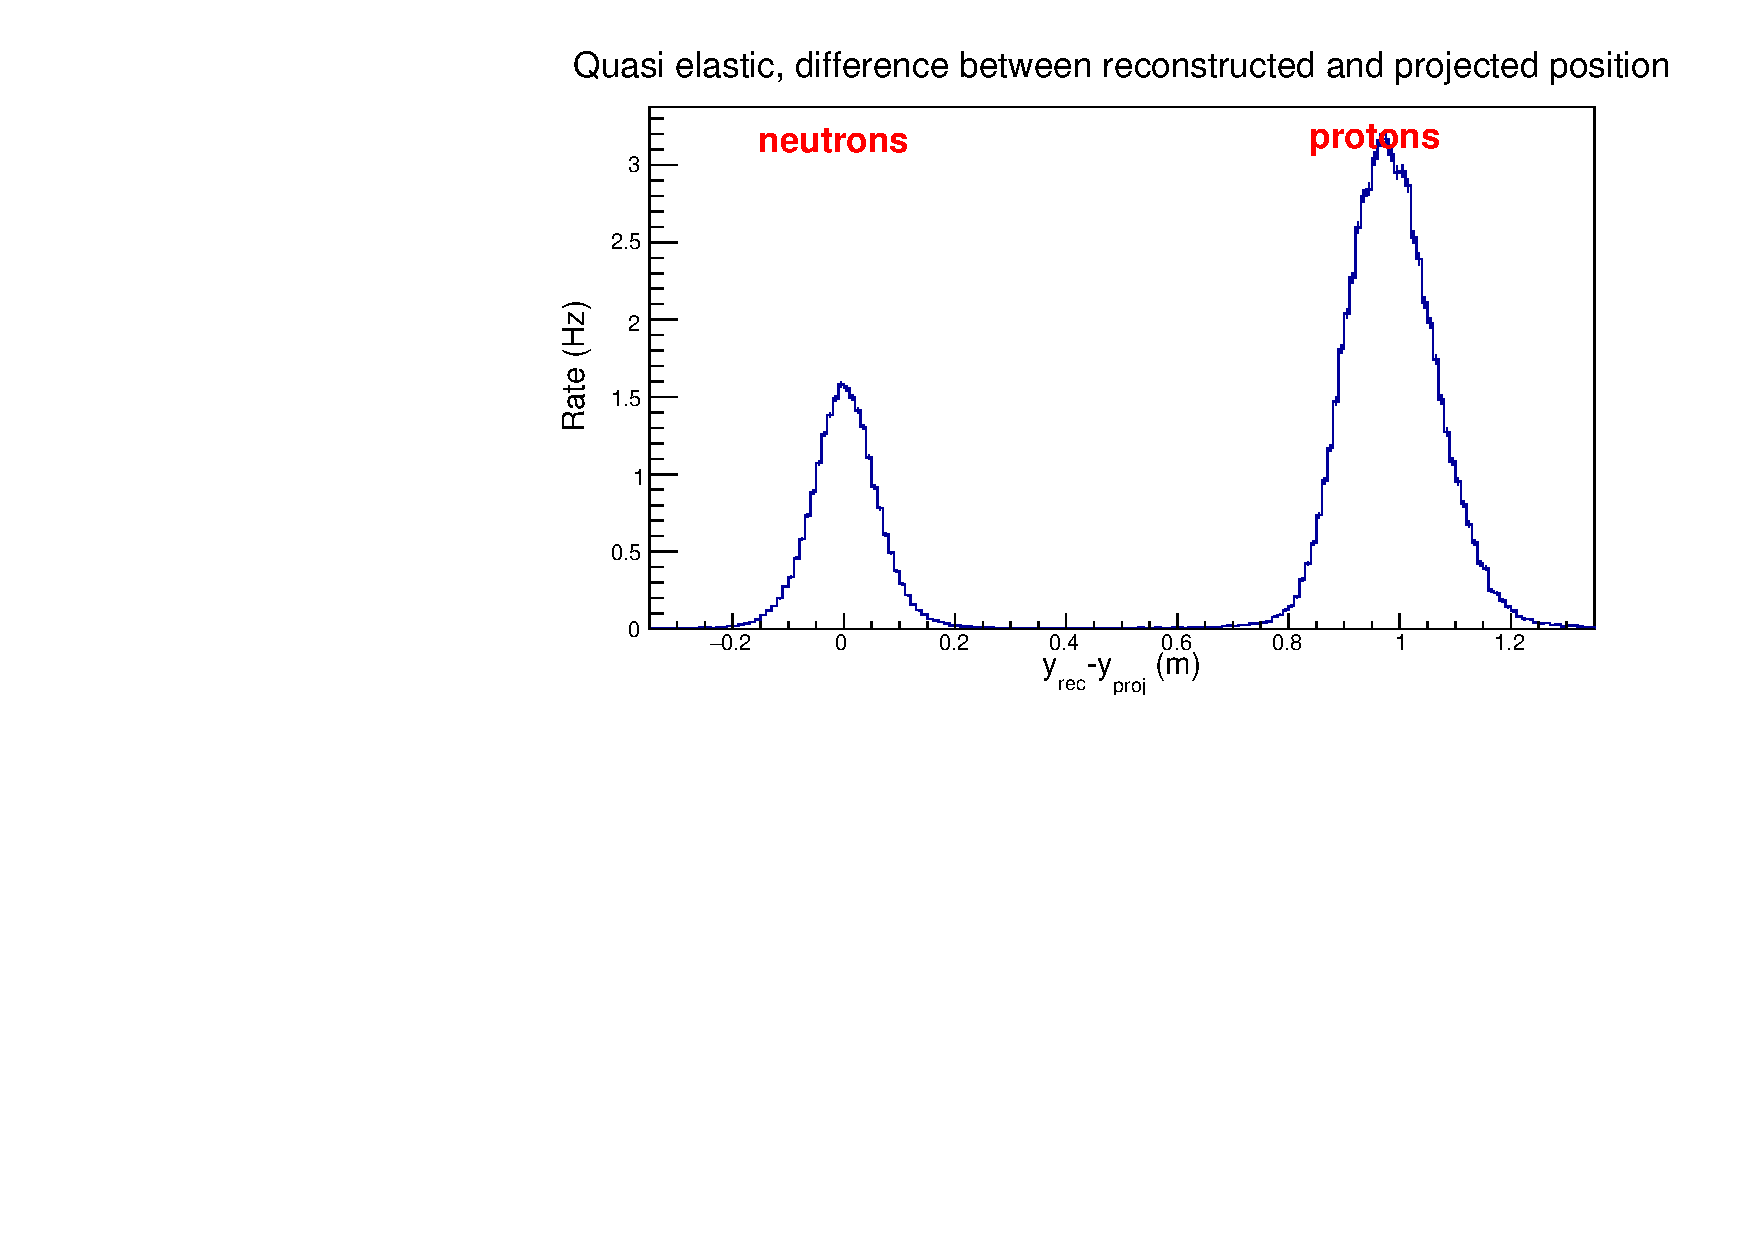
\includegraphics[width=6cm]{HCal_PID_QE_y.pdf}
    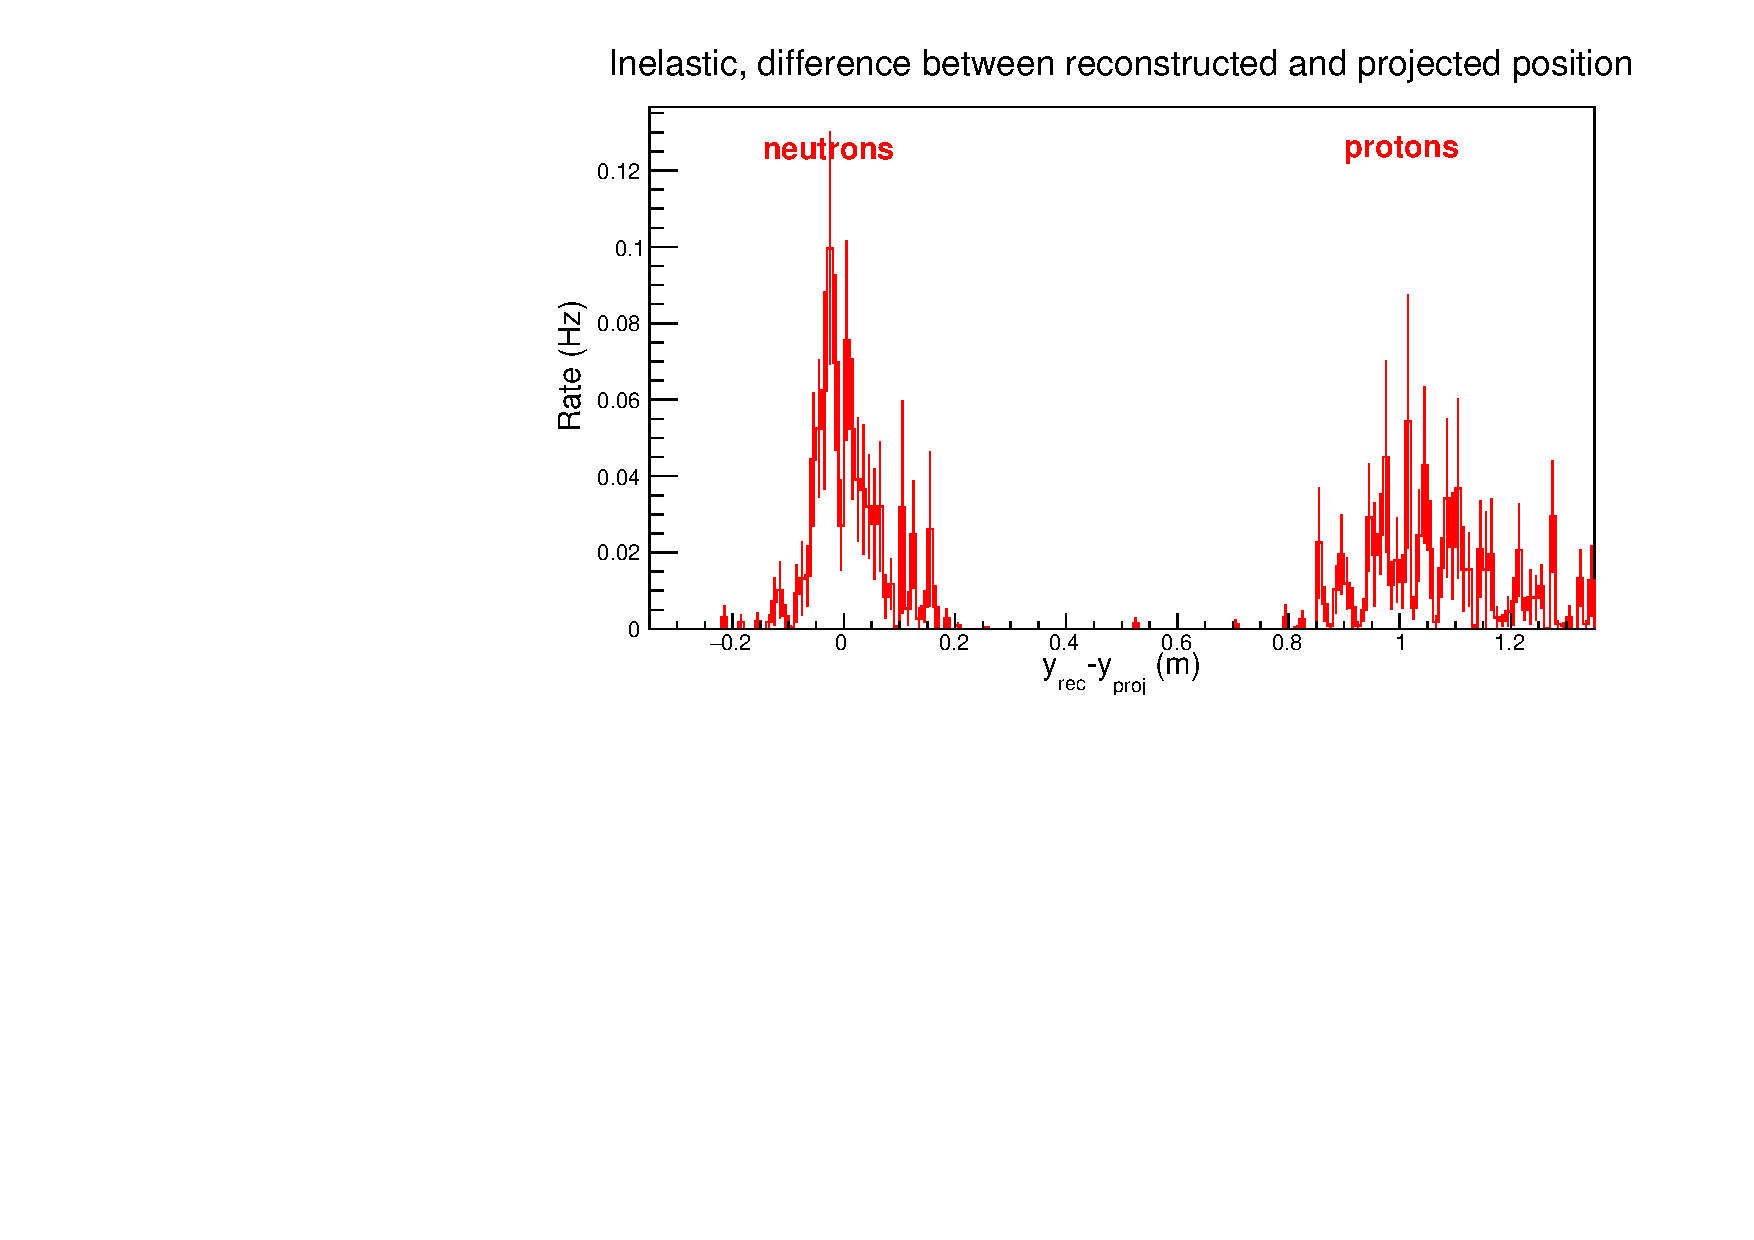
\includegraphics[width=6cm]{HCal_PID_Inel_y.pdf}
    \caption{Difference of projected position and reconstructed position for the nucleons projected in $y$ (dispersive direction), compared between quasi-elastic (left) and inelastic (right) events. The selection for these distributions are the fiducial cuts $W^2<1.10~{\rm GeV}^2$. We may notice that the selection on $W^2<1.10~{\rm GeV}^2$ already reduces drastically the proportion of inelastic with respect to quasi elastic. We may also see that the distribution for the proton is slightly wider. %, which will induce a slight decrease in $e-p$ events, which is fully calculable.
    }
    \label{hcal_id_y}
\end{figure}
%

As a second step, for the nucleons identified as protons (based on the location of the HCal cluster position with respect to its projected position), we need to correct the HCal reconstructed position $y_{rec}$ by the average shift $\Delta y_{p, avg}$ observed in figure~\ref{hcal_id_2D} for the nucleons identified as protons.

%Then, the HCal cluster position can be combined with the vertex position to retrieve the nucleon scattering angle $\theta_N$.
The nucleon momentum norm $p' = |\vec{p'}|$ is assumed to be equal to the virtual photon norm $|\vec{q}|$.
With this information we can calculate the proton shift $\Delta y_{p}$ for each proton.
%evaluated assuming the elastic scattering on a free nucleon, using the relation between the nucleon scattering angle and momentum in elastic scattering: $\vec{q}$
%$p' = 2M_N E (M_n+E cos(\theta_N)/(M_N^2+2M_N E+(E \sin{\theta_N}^2)$, with $E$ the beam energy and $M_N$ the nucleon mass.

With this information we may build the transverse components of the nucleon momentum (in the SBS coordinates system) $p'_{x, SBS}$ and $p'_{y, SBS}$.
For both the protons and neutrons, $p'_{x, SBS}$ can be written as $p'_{x, SBS} = p' \times (x_{rec}-v\sin{\theta_{SBS}})/(D_{HCal}-v\cos{\theta_{SBS}})$ (with $v$ the reconstructed vertex position, $D_{HCal}$ the HCal distance to the target and $\theta_{SBS}$ the spectrometer angle.
For the neutrons, $p'_{y, SBS}$ is $p'_{y, SBS} = p' \times y_{rec}/(D_{HCal}-v\cos{\theta_{SBS}})$.
For the protons, $p'_{y, SBS}$ must be written as $p'_{y, SBS} = p' \times (y_{rec} - \Delta y_{p})/(D_{HCal}-v\cos{\theta_{SBS}})$.

The nucleon momentum components in the SBS coordinates system $p'_{x, SBS}$ and $p'_{y, SBS}$ can then be transformed (using the corrected HCal distance to the target $D_{HCal}-v\cos{\theta_{SBS}}$) into the nucleon momentum components in the Hall~A coordinate system $p'_{x}$, $p'_y$ and $p'_z$, with the best resolution achievable. 

In Hall~A coordinate system, using the nucleon meomentum combined with the virtual photon vector $\vec{q}$, we may reconstruct the transverse missing momentum $p_{_{\perp} miss} = \sqrt{(q_{x}-p'_{x})^2+(q_{y}-p'_{y})^2}$, which is another very powerful variable to reject more inelastic background.
Figure~\ref{fig:pperp} displays the event distributions in $p_{_{\perp} miss}$ for our simulated quasi-elastic sample within our fiducial acceptance cuts%, but before requiring $W^2<1.10~{\rm GeV}^2$.
, and requiring $W^2<1.10~{\rm GeV}^2$.
%
\begin{figure}[h]
  \centering
    %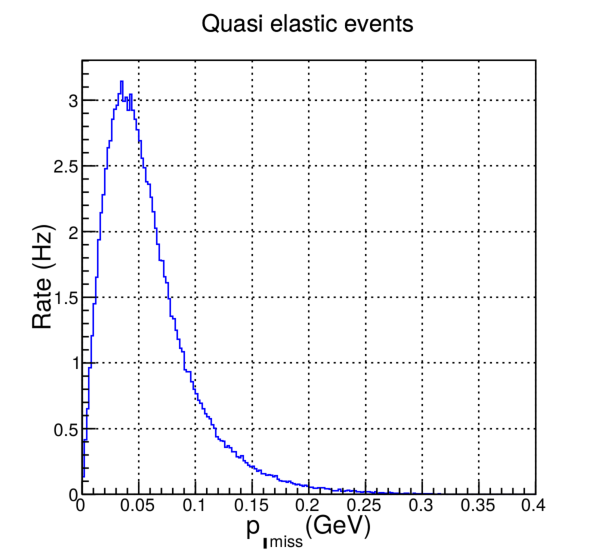
\includegraphics[width=5cm]{pperp_sig.pdf}
    %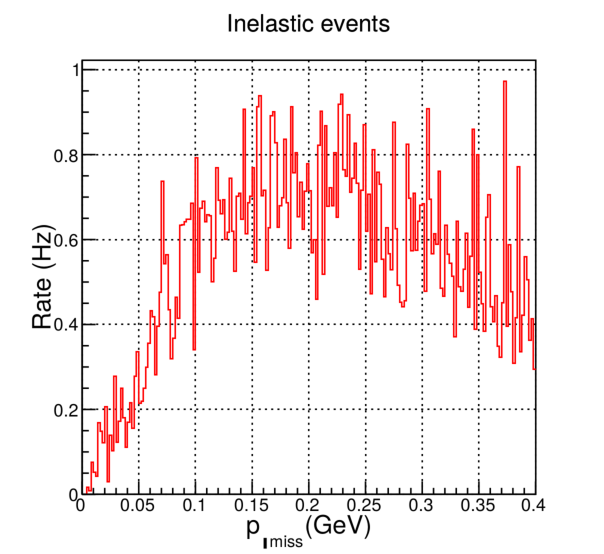
\includegraphics[width=5cm]{pperp_inel.pdf}
    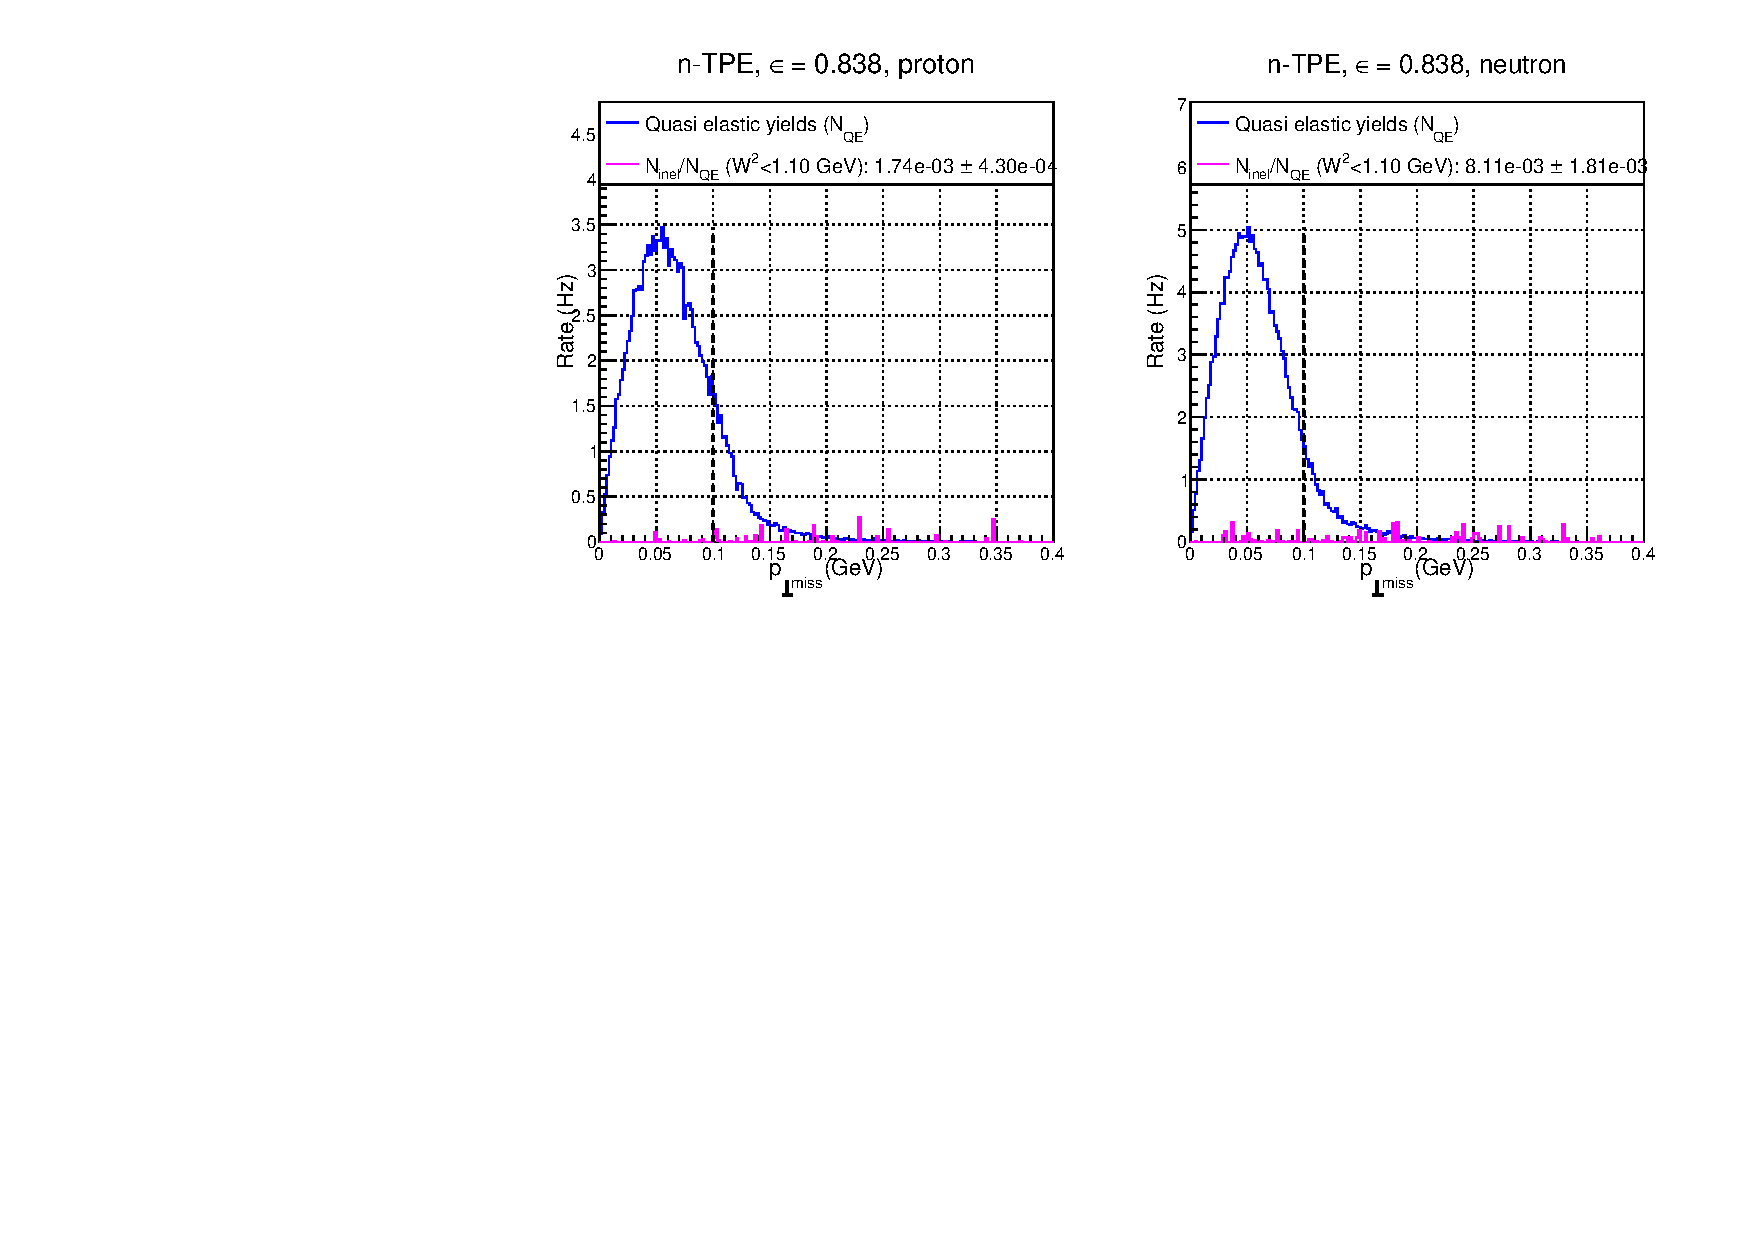
\includegraphics[width=12cm]{gen-tpe_he_pperp_acc_real_new.pdf}
    %\caption{Event distributions in $p_{_{\perp} miss} = \sqrt{(q_{x}-p'_{x})^2+(q_{y}-p'_{y})^2}$ for quasi elastic $e-N$ (left) and inelastic resonant $e-N$ (right) within the fiducial analysis cuts, but before requiring $W^2<1.10~{\rm GeV}^2$.}
    \caption{Compared quasi-elastic (blue) and inelastic (magenta) distributions for $p_{_{\perp} miss} = \sqrt{(q_{x}-p'_{x})^2+(q_{y}-p'_{y})^2}$, within fiducial analysis cuts, after requiring $W^2<1.10~{\rm GeV}^2$, for the high $\epsilon$ kinematic, separated between protons on the left and neutrons on the right). The inelastic contamination of quasi-elastic events and their error bars are quoted in the legends.}
    \label{fig:pperp}
\end{figure}
%
%After applying $W^2<1.10~{\rm GeV}^2$ 
After selection on $W^2 <1.10 {\rm GeV}^2$ and $p_{_{\perp} miss} <0.1$~GeV, the inelastic contamination of our quasi-elastic sample is better than 1\%, with 0.2\% systematic uncertainties.

\iffalse
%, and the missing transverse momentum $p_{_{\perp} miss}$ between the reconstructed nucleon $p'$ and the reconstructed virtual photon $q$ such as $p_{_{\perp} miss} = \sqrt{(q_{x}-p'_{x})^2+(q_{y}-p'_{y})^2}$.
The nucleon is reconstructed using the position of the HCal cluster which, combined with the vertex position, allows to retrieve the nucleon scattering angle $\theta_N$.
The nucleon momentum is then evaluated assuming elastic scattering on a free nucleon, using the relation between the nucleon scattering angle and momentum in elastic scattering:
$p' = 2M_N E (M_n+E cos(\theta_p)/(M_N^2+2M_N E+(E \sin{\theta_p}^2)$, with $E$ the beam energy and $M_N$ the nucleon mass.


%(2*M_N*k0*(M_N+k0)*cos(thetap))/(M_N*M_N+2*M_N*k0+pow(k0*sin(thetap),2));
%With 0.5 ns time resolution 
%For a 3.2 GeV/c nucleon, 

Figure~\ref{fig:qe} display the event distributions in those variables for our simulated quasi-elastic sample within the following set of cuts:
%
\begin{itemize}
\item{the electron track is reconstructed in BigBite;}
\item{the total energy deposited in the BigBite calorimeter is above 3 GeV (resp. 1.3 GeV) set for 95\% of the 4.2 GeV (resp. 2 GeV) elastic peak for the high (resp. low) $\epsilon$ kinematic;}
\item{the electron track must fire at least 3 PMTs in the GRINCH detectors;}
\item{the total energy deposited in HCal is 0.1 GeV, set for 90\% efficiency of the 0.2 GeV deposited by the 3.2 GeV/c nucleons in the HCal scintillator material.}
\end{itemize}
%
\begin{figure}[h]
  \centering
    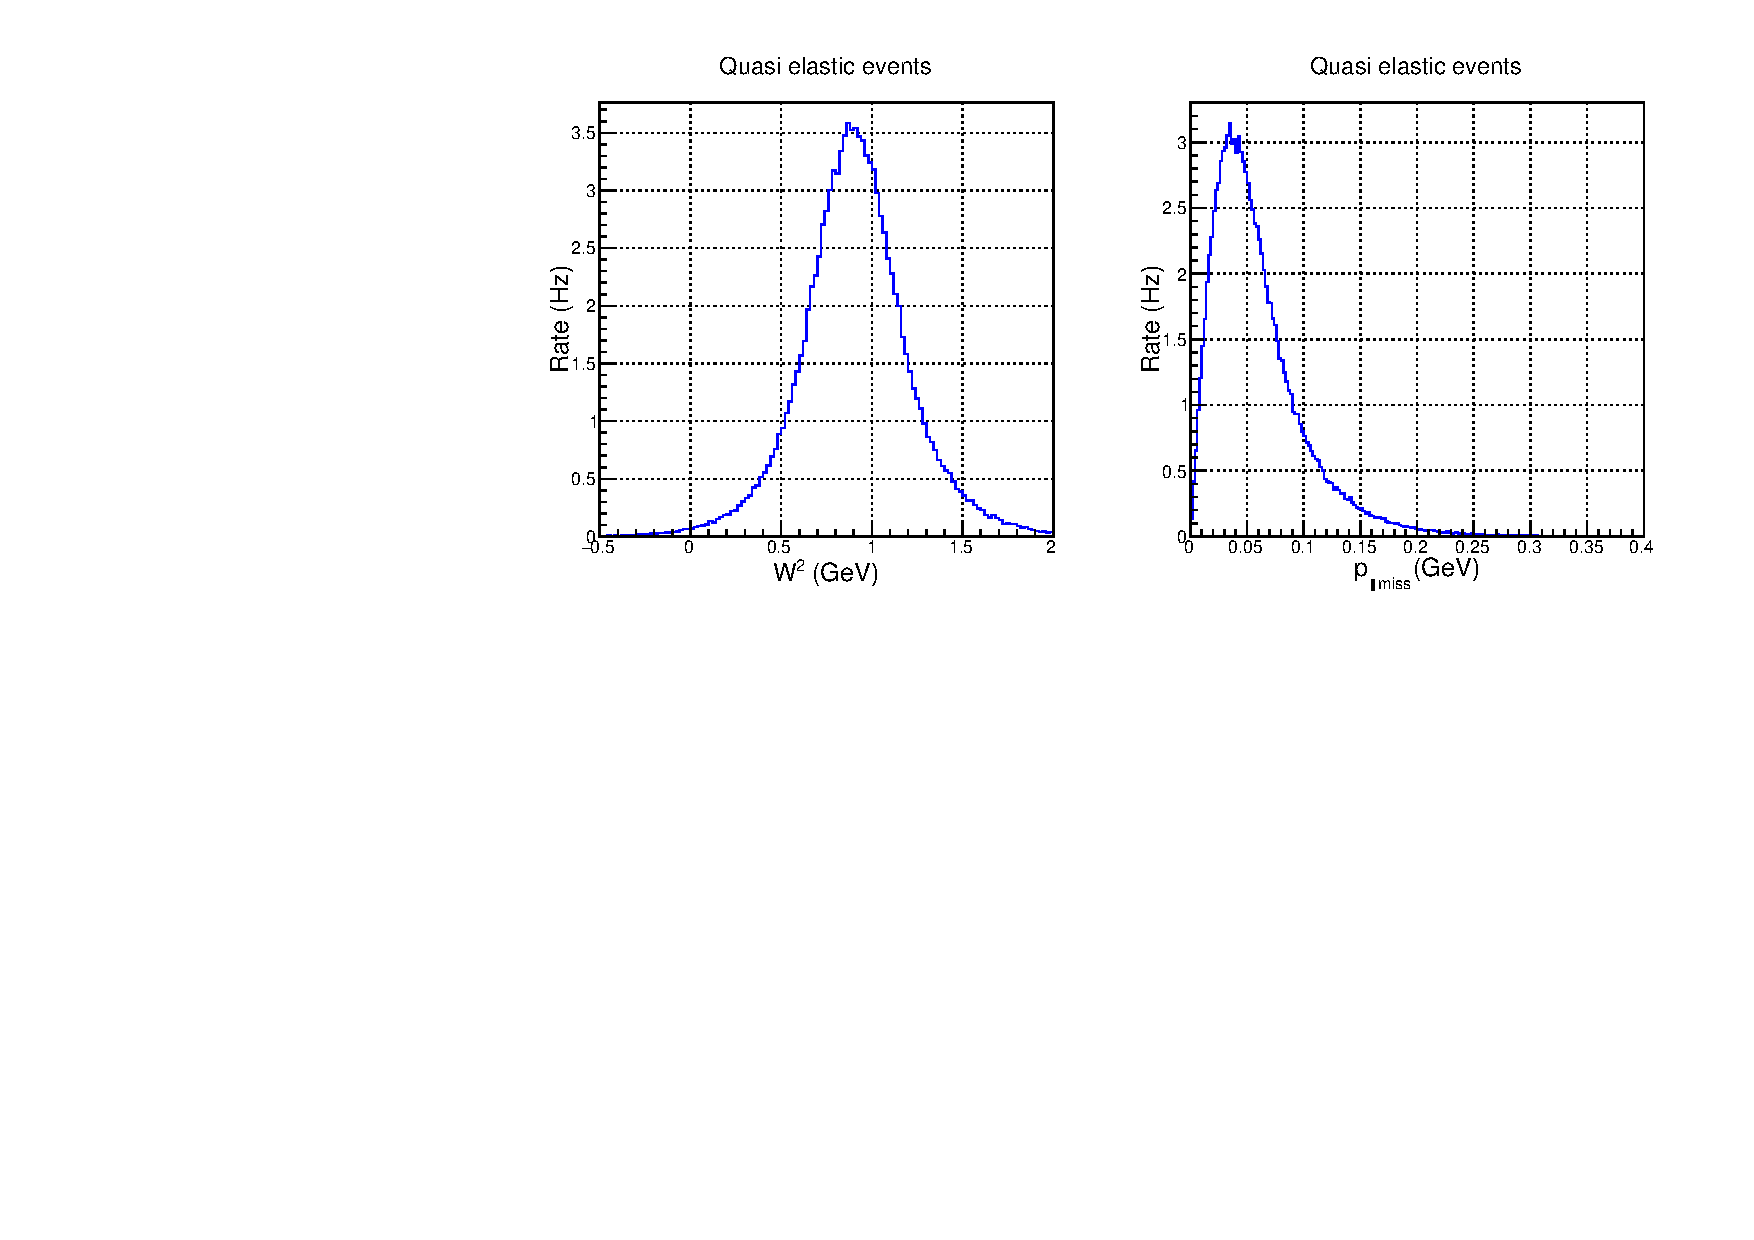
\includegraphics[width=10cm]{W2_pperp_sig.pdf}
    \caption{Quasi-elastic event distributions in $W^2 = M_{N}^2+2M_{N}^{2}(E-E')-Q^2$ (left) and $p_{_{\perp} miss} = \sqrt{(q_{x}-p'_{x})^2+(q_{y}-p'_{y})^2}$ (right), within the fiducial analysis cuts.}
    \label{fig:qe}
\end{figure}
%
Figure~\ref{fig:inel} display the event distributions in those variables for our simulated inelastic resonant $e-N$ scattering.
%
\begin{figure}[!h]
  \centering
    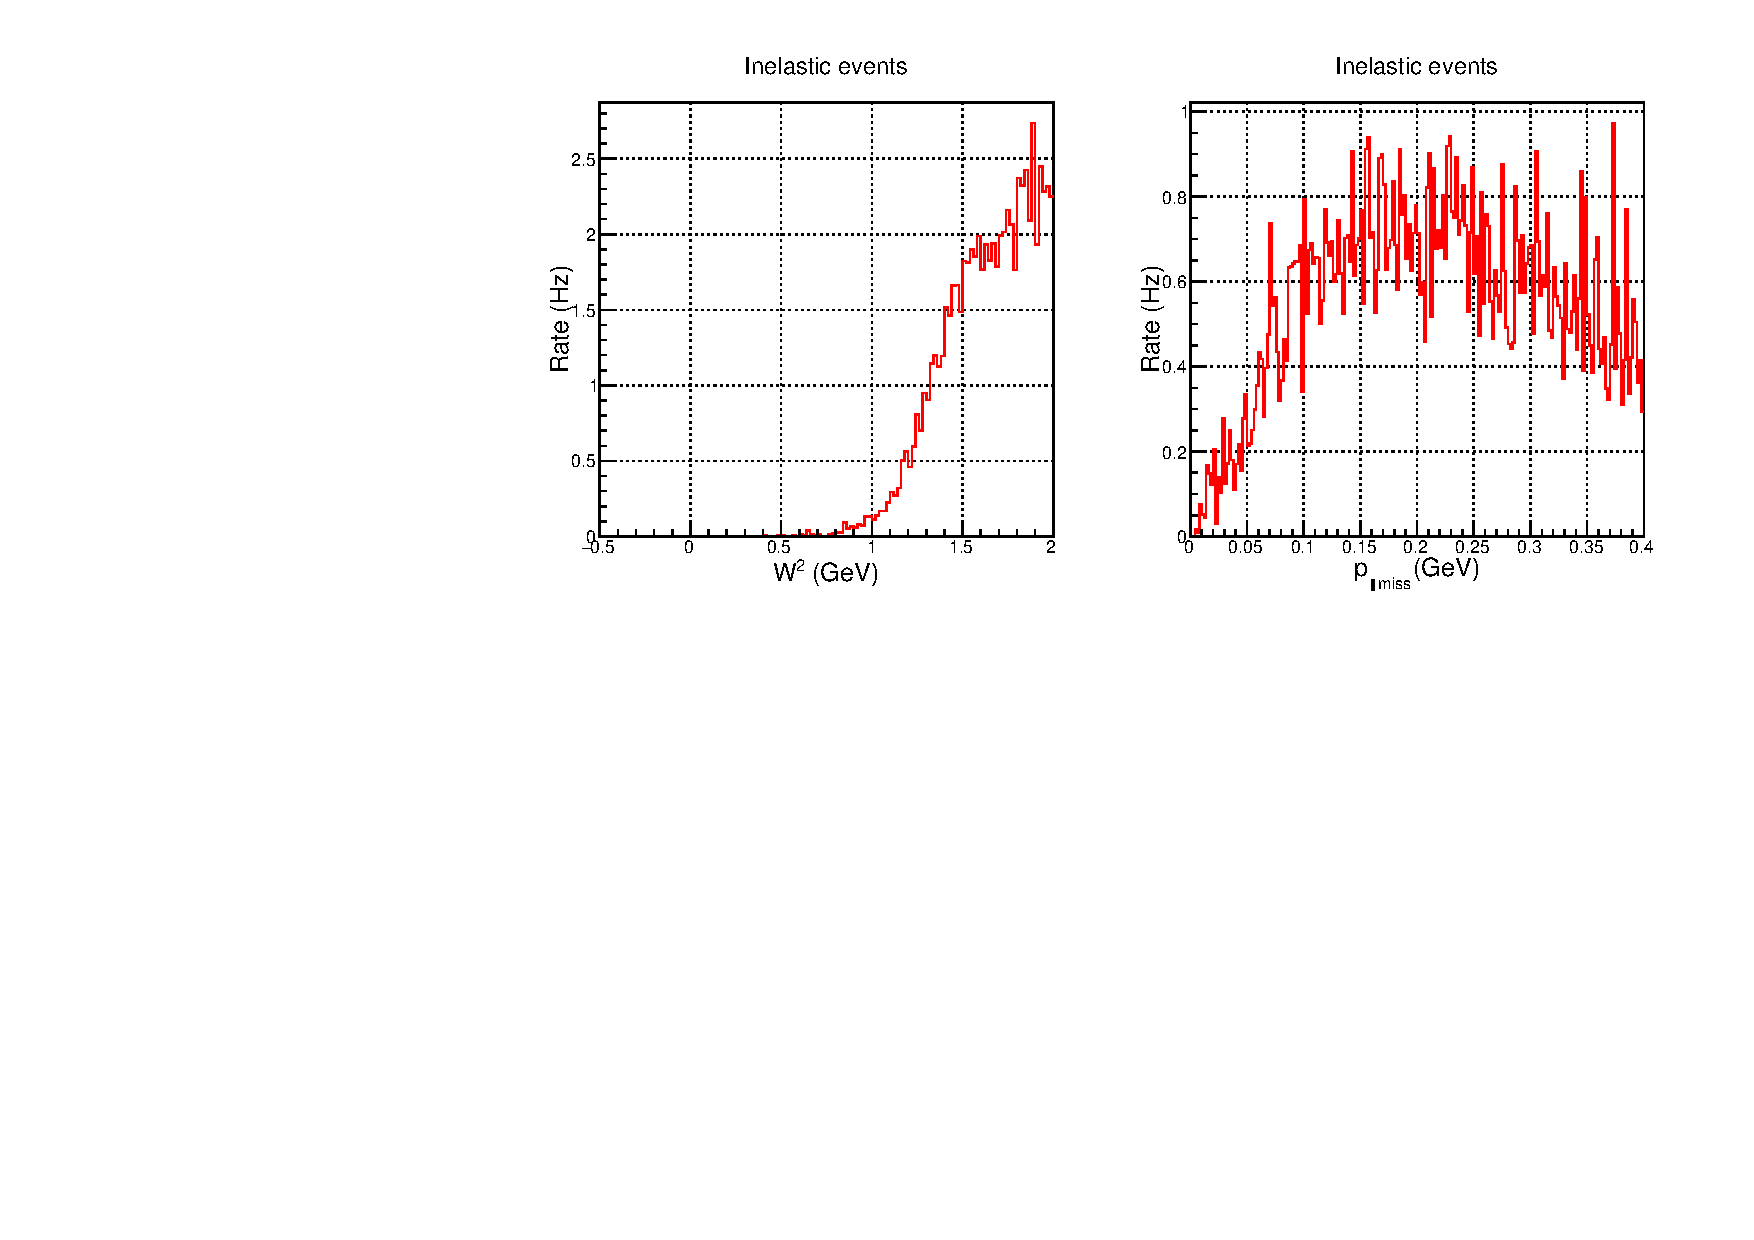
\includegraphics[width=10cm]{W2_pperp_inel.pdf}
    \caption{Inelastic resonant $e-N$ distributions for $W^2 = M_{N}^2+2M_{N}^{2}(E-E')-Q^2$ (left) and $p_{_{\perp} miss} = \sqrt{(q_{x}-p'_{x})^2+(q_{y}-p'_{y})^2}$ (right), within the fiducial analysis cuts.}
    \label{fig:inel}
\end{figure}
%

After selection on $W^2 <1.10~{\rm GeV}^2$ and $p_{_{\perp} miss} <0.1$~GeV, we select the protons and neutrons, based on the difference between their reconstructed position and their projected position (see figure~\ref{hcal_id}).
%
\begin{figure}[!h]
  \centering
    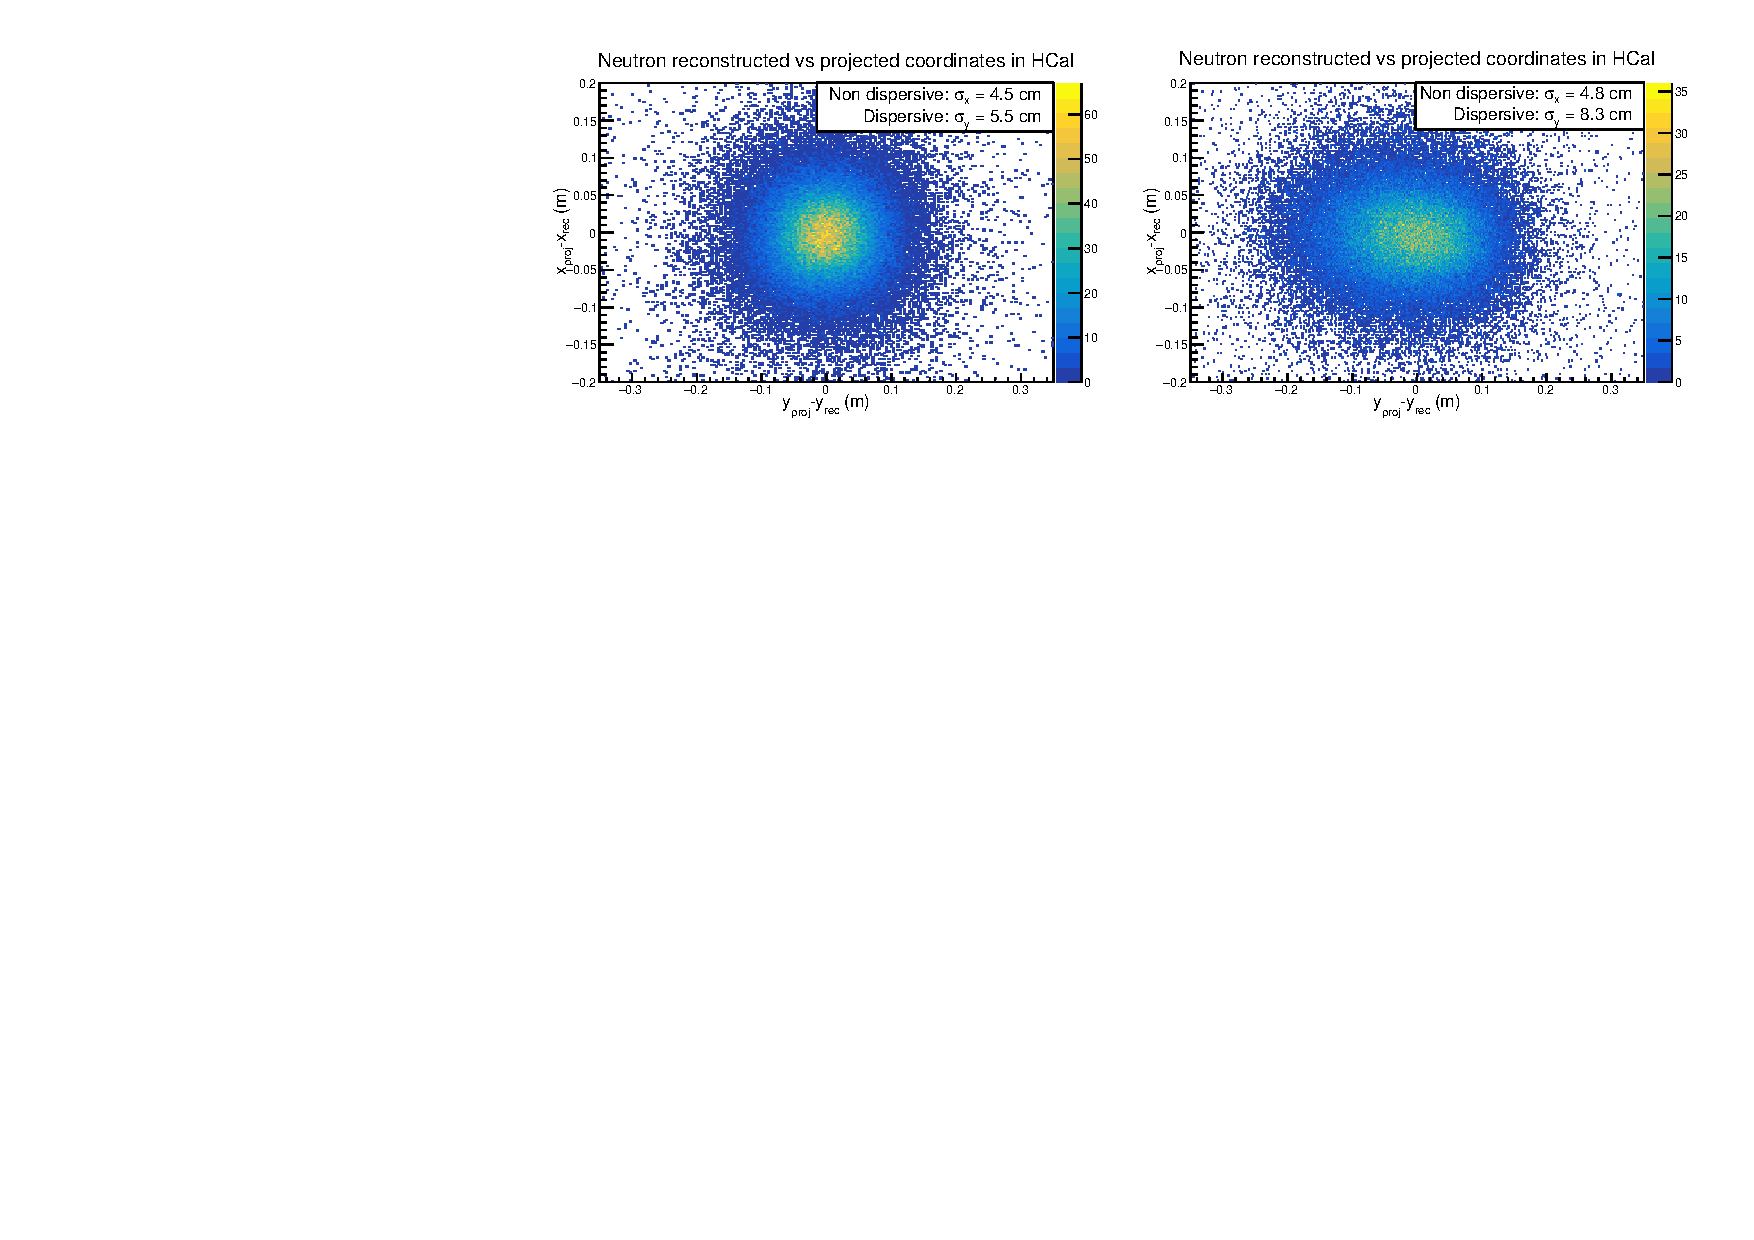
\includegraphics[width=10cm]{HCal_PID.pdf}
    \caption{Reconstructed Vs projected position of the neutrons (left) and the protons(right) in HCal. In the analysis a hadron is identified as a proton (resp. neutron) when it is reconstructed 3$\sigma$ of its projected position in both $x$ and $y$.}
    \label{hcal_id}
\end{figure}
%
After the hadron identification, we evaluate our inelastic contamination for the separated proton and neutron yield events.
Figure~\ref{fig:inel_contam_le} (resp. \ref{fig:inel_contam_he} ) shows $p_{_{\perp} miss}$ distributions for the quasi-elastic and inelastic events after a selection on $W^2<1.10~{\rm GeV}^2$ for the low $\epsilon$ (resp. high $\epsilon$) kinematics. The inelastic contamination of quasi-elastic events for $p_{_{\perp} miss} < 0.1$ GeV (quoted on the legends of figures~\ref{fig:inel_contam_le} and \ref{fig:inel_contam_he}) are below 1\%, with an absolute uncertainty below 0.2\%. 
%
\begin{figure}[!h]
  \centering
    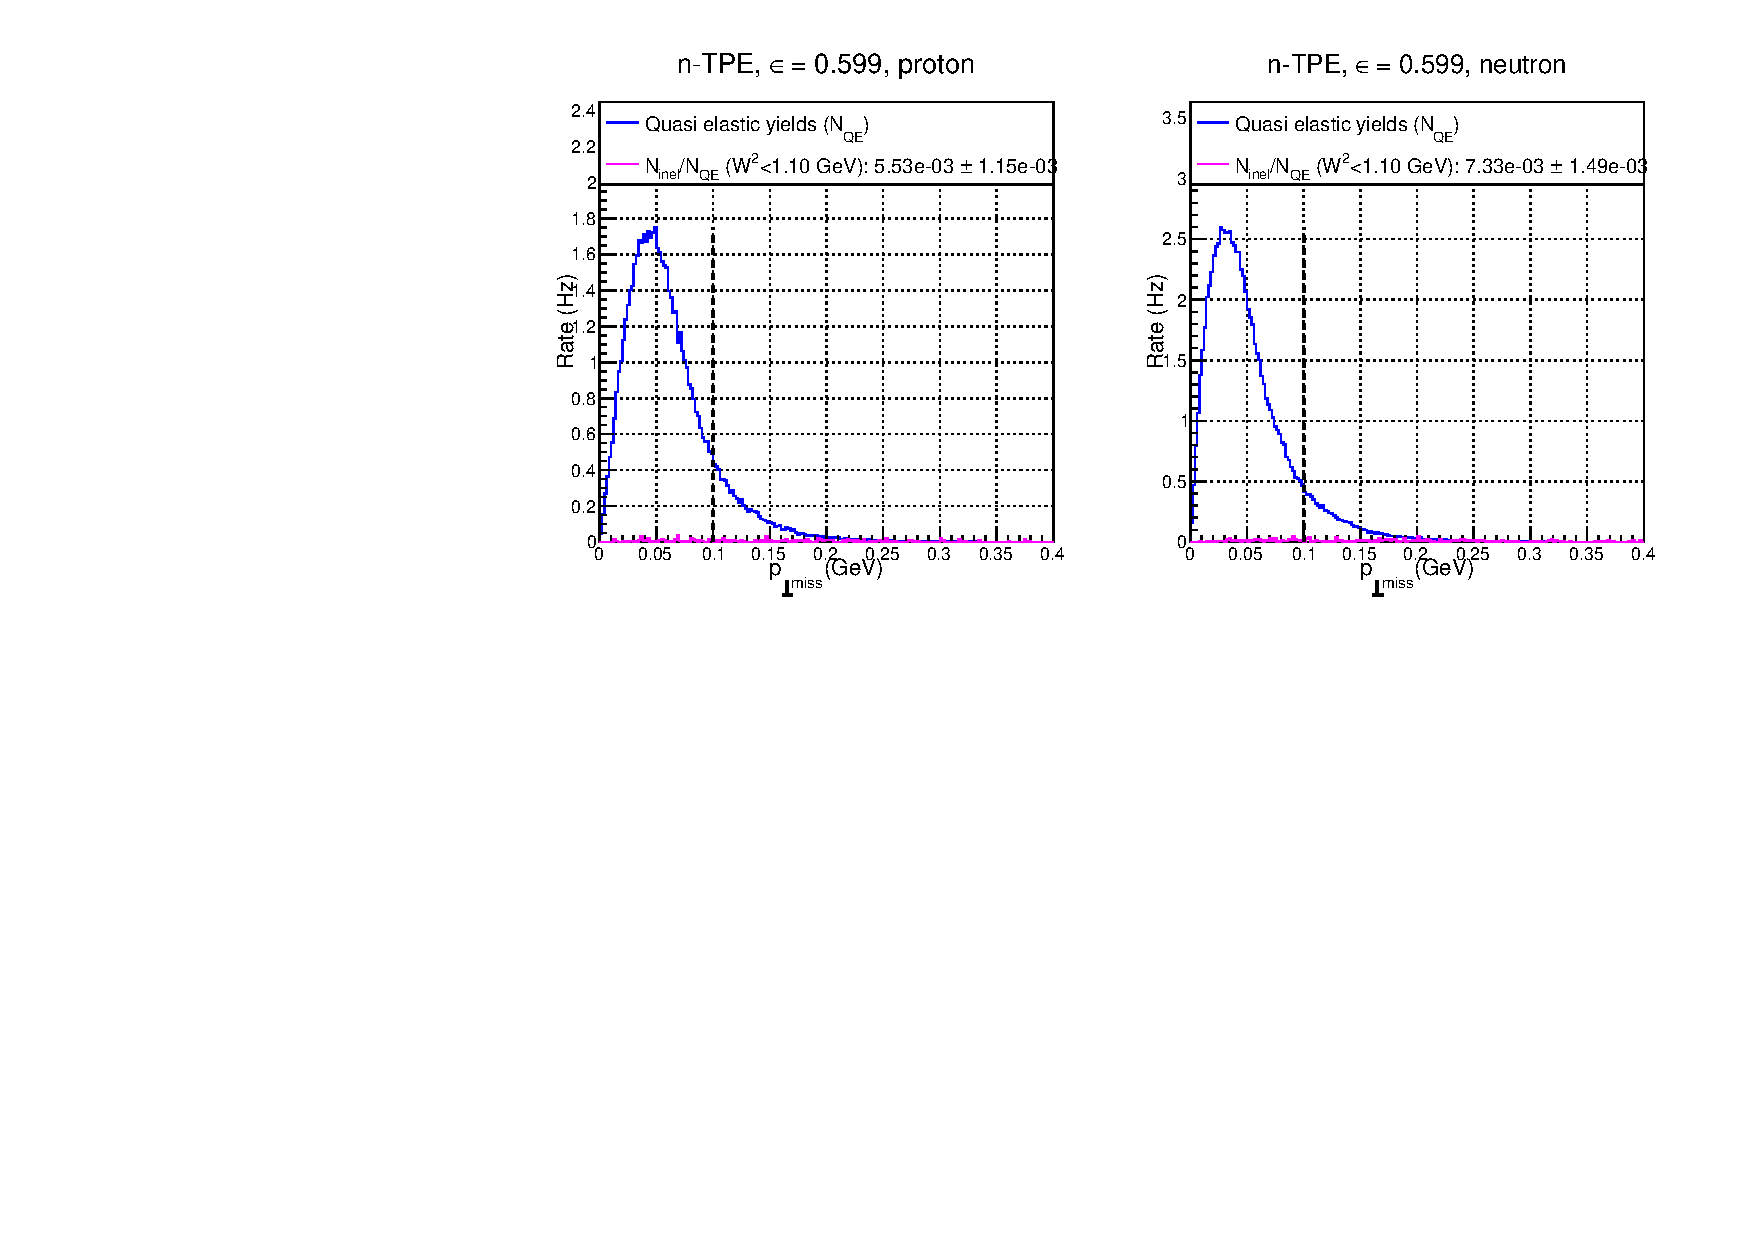
\includegraphics[width=12cm]{gen-tpe_le_pperp_acc_real_new.pdf}
    %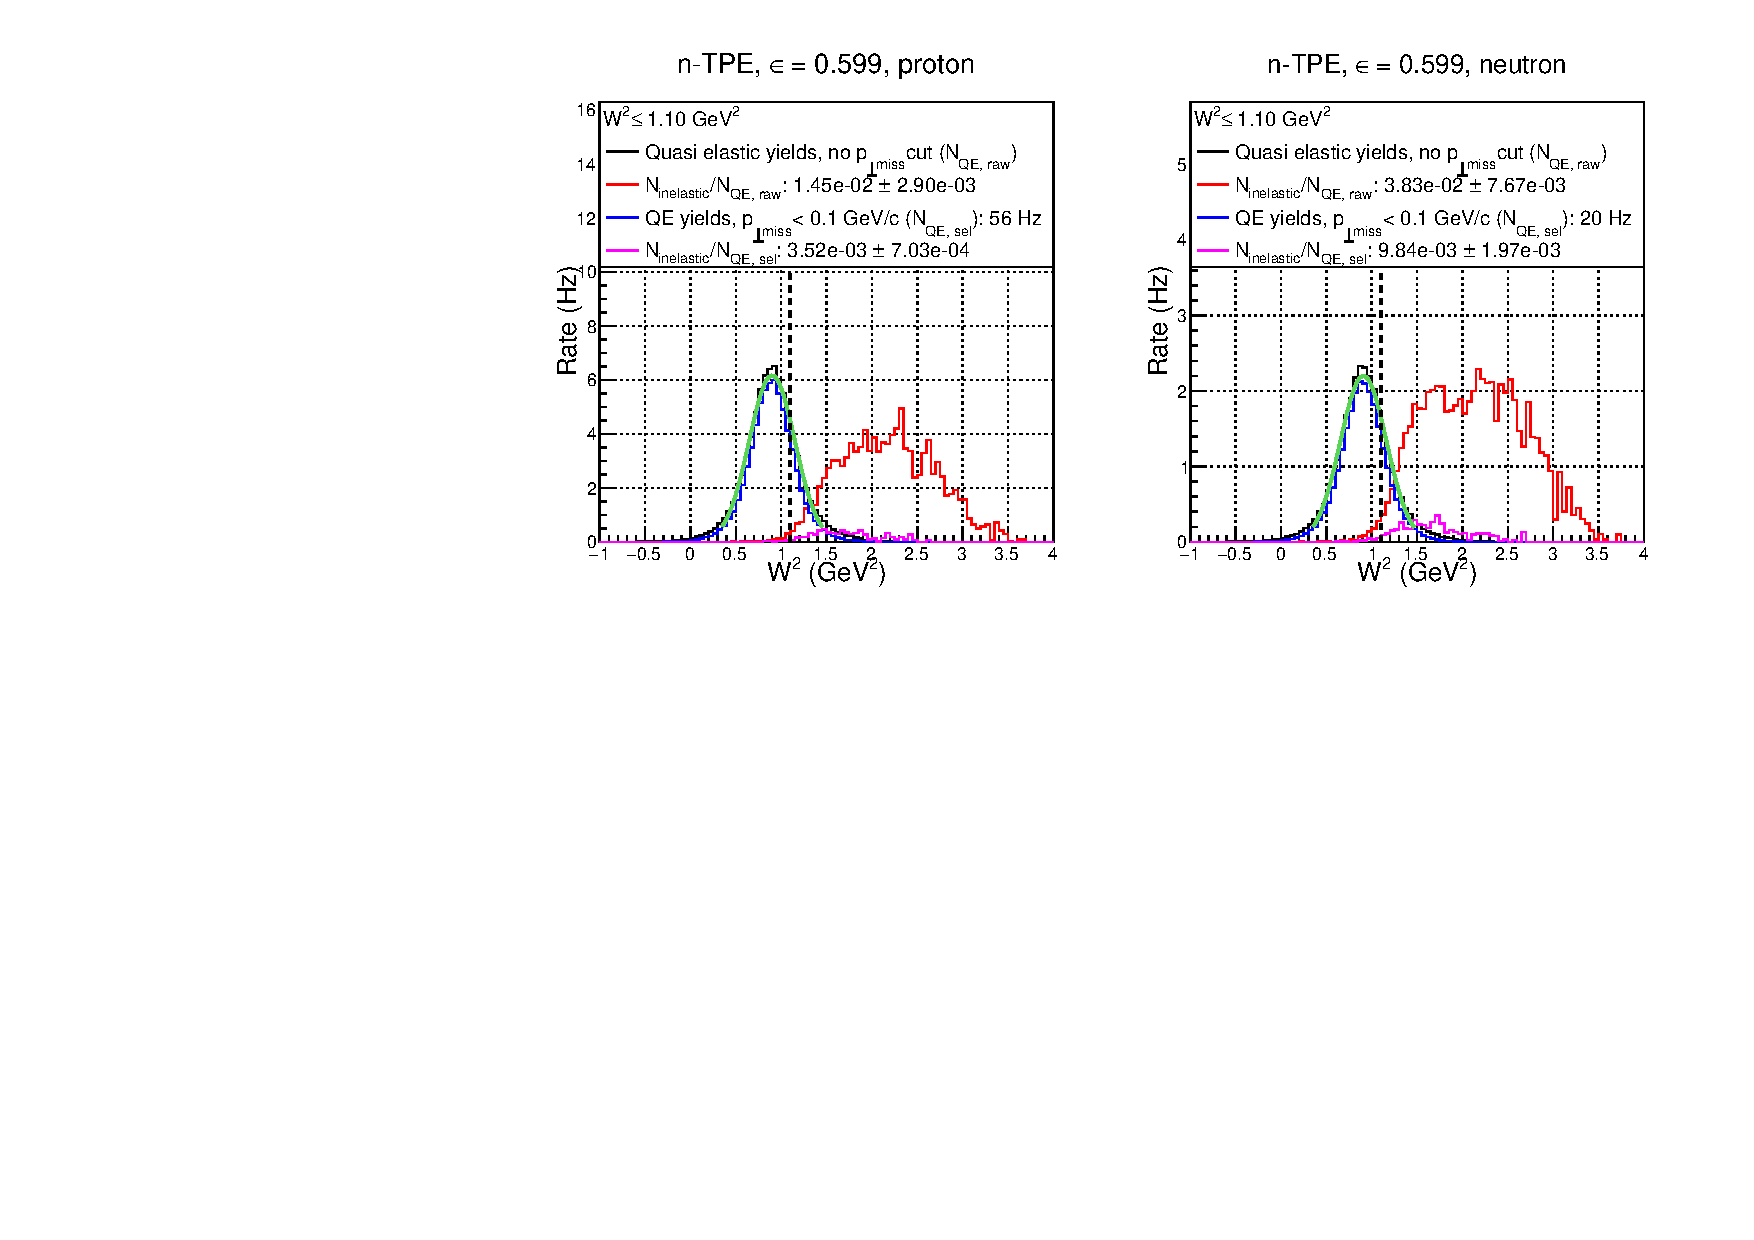
\includegraphics[width=12cm]{gen-tpe_le_W2_acc_real.pdf}
    \caption{Compared quasi-elastic and inelastic distributions (including detectors resolutions) for $p_{_{\perp} miss} = \sqrt{(q_{x}-p'_{x})^2+(q_{y}-p'_{y})^2}$, within fiducial analysis cuts, for the low $\epsilon$ kinematic. The inelastic contamination of quasi-elastic events and their error bars are quoted in the legends. Comparison for protons (resp. neutrons) is shown on the left (resp. on the right).}%Compared quasi-elastic and inelastic distributions (including detectors resolutions) for $p_{_{\perp} miss} = \sqrt{(q_{x}-p'_{x})^2+(q_{y}-p'_{y})^2}$ (top) and $W^2 = M_{N}^2+2M_{N}^{2}(E-E')-Q^2$ (bottom), within fiducial analysis cuts, for the low $\epsilon$ kinematic. The inelastic contamination of quasi-elastic events and their error bars are quoted in the legends. Comparison for protons (resp. neutrons) is shown on the left (resp. on the right). On the bottom panel, black and red are before the $p_{_{\perp} miss}~\leq~0.1~\mathrm{GeV}$ selection, while blue and magenta are after $p_{_{\perp} miss}~\leq~0.1~\mathrm{GeV}$ selection.}
    \label{fig:inel_contam_le}
\end{figure}
%
\begin{figure}[!h]
  \centering
    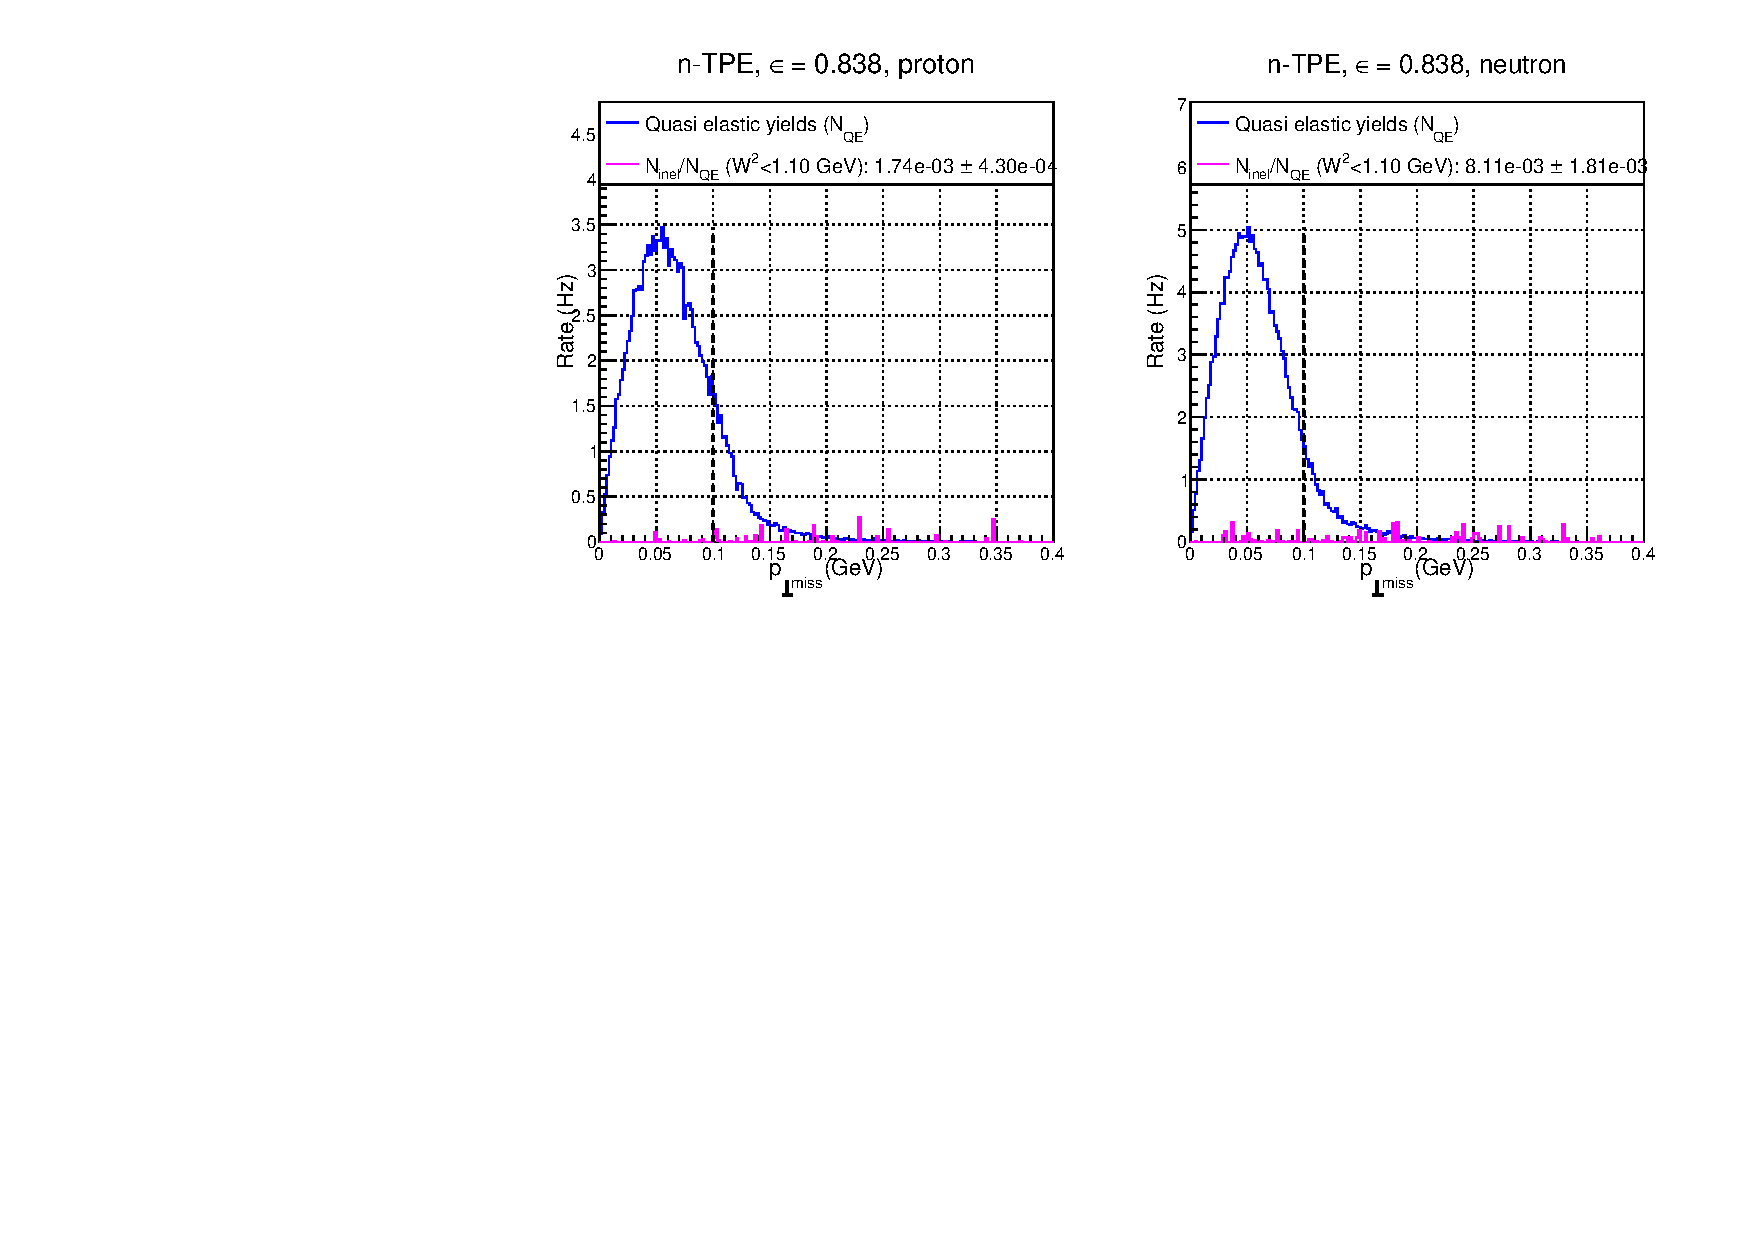
\includegraphics[width=12cm]{gen-tpe_he_pperp_acc_real_new.pdf}
    %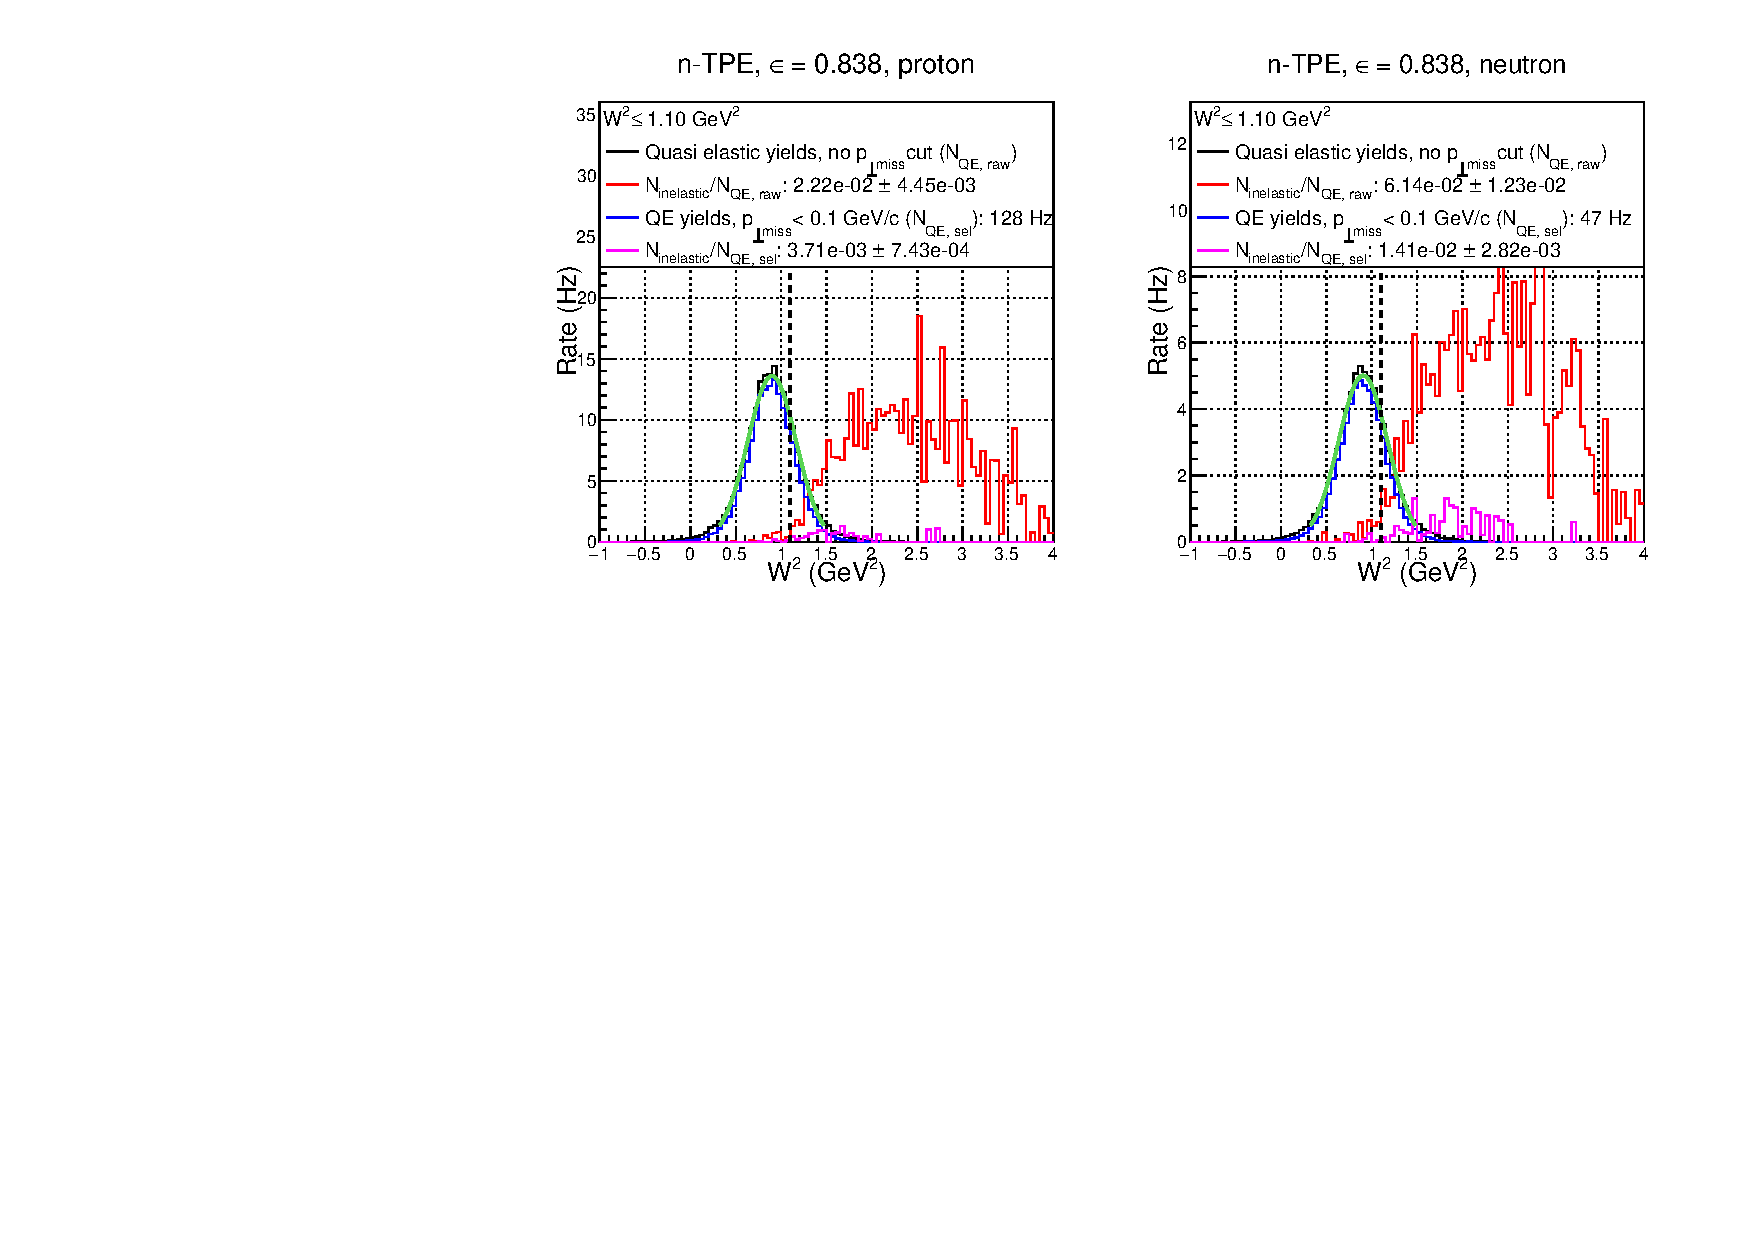
\includegraphics[width=12cm]{gen-tpe_he_W2_acc_real.pdf}
    \caption{Compared quasi-elastic and inelastic distributions (including detectors resolutions) for $p_{_{\perp} miss} = \sqrt{(q_{x}-p'_{x})^2+(q_{y}-p'_{y})^2}$, within fiducial analysis cuts, for the high $\epsilon$ kinematic. The inelastic contamination of quasi-elastic events and their error bars are quoted in the legends. Comparison for protons (resp. neutrons) is shown on the left (resp. on the right).}%Compared quasi-elastic and inelastic distributions (including detectors resolutions) for $p_{_{\perp} miss} = \sqrt{(q_{x}-p'_{x})^2+(q_{y}-p'_{y})^2}$ (top) and $W^2 = M_{N}^2+2M_{N}^{2}(E-E')-Q^2$ (bottom), within fiducial analysis cuts, for the high $\epsilon$ kinematic. The inelastic contamination of quasi-elastic events and their error bars are quoted in the legends. Comparison for protons (resp. neutrons) is shown on the left (resp. on the right). On the bottom panel, black and red are before the $p_{_{\perp} miss}~\leq~0.1~\mathrm{GeV}$ selection, while blue and magenta are after $p_{_{\perp} miss}~\leq~0.1~\mathrm{GeV}$ selection and application of BigBite shower and HCal thresholds.}
    \label{fig:inel_contam_he}
\end{figure}
%
\fi
The nucleon time-of-flight information can also be used to further suppress background. The HCal time resolution of 0.5 ns allows to resolve time-of-flight for 3.2 GeV/c nucleons with 12\% resolution.

In addition, the level of inelastic contamination reported in the document are for the en and ep yields.
The observable we are interested in is the {\it ratio} $N_{en}/N_{ep}$, in which the inelastic contribution partly cancels.
The cancellation is not complete because the fractional errors in the numerator and 
denominator will differ.
But the partial cancellation results in a fractional error on the ratio which is smaller than the fractional error contributed to the neutron or proton counts.
In addition, in the (likely) event that we underestimate our background contamination,
we expect to underestimate it by the same amount for $e-p$ and $e-n$, so the point above remains true.\\

\iffalse
The contribution of inelastic in the final statistics is very small (less than 2\% at most).
Figures~\ref{fig:inel_contam_le} and \ref{fig:inel_contam_he} show event distributions the quasi-elastic and inelastic distributions of $p_{_{\perp} miss} = \sqrt{(q_{x}-p'_{x})^2+(q_{y}-p'_{y})^2}$ and $W^2 = M_{N}^2+2M_{N}^{2}(E-E')-Q^2$ reconstructed within our fiducial analysis cuts.
The fiducial cuts are defined as:
%
\begin{itemize}
\item{the electron track is reconstructed in BigBite, and the vertex is;}
\item{the total energy deposited in the BigBite calorimeter above the threshold defined for this detector: 3 GeV for 4.2 GeV elastic peak for the high $\epsilon$ kinematic, 1.32 GeV for 2 GeV elastic peak for the low $\epsilon$ kinematic.}
\item{the track will fire at least 3 PMTs in the GRINCH detectors;}
\item{the total energy deposited in the hadron calorimeter is above the threshold defined for this detector.}
\end{itemize}
%
Figures~\ref{fig:inel_contam_le},~\ref{fig:inel_contam_he} also quote the actual inelastic contamination values of quasi-elastics with error bars).
For the inelastic cross section, we used the model by P.~Bosted and E.~Christy\footnote{Phys.~Rev.~C81.055213, https://arxiv.org/abs/0712.3731}. See also the GMn E12-09-019 proposal page (attached).
This model is a fit of $e-N$ data in the resonance region from Jefferson Lab Hall C\footnote{http://arxiv.org/abs/nucl-ex/0410027} which covers $0<=Q^2<8 {GeV/c}^2$, with beam energies up to 5.5 GeV.

According to $^2$, %\footnote{Phys.~Rev.~C81.055213, https://arxiv.org/abs/0712.3731},
the fit residue to the data between 4 and 6 GeV fluctuates by $\pm$ 10\%. We assume a 20\% systematic error attached on our inelastic background estimation or 0.4\% relative quasi-elastic.


In addition, the level of inelastic contamination reported in the document are for
the en and ep yields.
The observable we are interested in is the {\it ratio} $N_{en}/N_{ep}$, in which the inelastic contribution partly cancels.
The cancellation is not complete because the fractional errors in the numerator and 
denominator will differ.
But the partial cancellation results in a fractional error on the ratio which is smaller than the fractional error contributed to the neutron or proton counts.
In addition, in the (likely) event that we underestimate our background contamination,
we expect to underestimate it by the same amount for ep and en, so the point above
remains true.\\
\fi

``The singles rate in HCal is huge and apparently the coincidence rate between BigBite and HCal is also large. How uncertain is the inelastic rate?''\\

%The single rates have been evaluated by beam-on-target Geant4 simulations, which

The inelastic background has been evaluated by Brian Quinn for the GMn experiment\footnote{https://www.jlab.org/exp\_prog/proposals/09/PR12-09-019.pdf}, see also CLAS GMn experiment\footnote{J.~Lachniet {\it et al.}, Phys.~Rev.~Lett.~102, 192001 (2009) https://arxiv.org/abs/0811.1716, see also Ph.D. thesis from CMU, 2005}.
Results from our analysis are in agreement with the previous results.\\
%The singles rates in HCal are very large;

%{\em private note: is he asking what is the inelastic rate in HCal? I'm not sure I understand...}\\

``You base it on a model, how valid is it for your needs?''\\

%\comment{repeat ``This model is a fit of $e-N$ data in the resonance region...''?}
As stated earlier, this model is a fit of $e-N$ data in the resonance region from Jefferson Lab Hall C$^{3}$ which covers $0<=Q^2<8~{\rm (GeV/c)}^2$, with beam energies up to 5.5 GeV. 
It may be argued that provided the data set on which this fit is based (for which
the beam energy is no higher than 5.5 GeV),
we might use it at the limit of its validity for our high $\epsilon$ point (for which
the beam energy is 6.6 GeV).\\

``How much of the inelastic tail do you measure, e.g. how much of Figs. 10 and 11 will come from data?''\\

On figure~\ref{fig:W2}, %\ref{fig:inel_contam_le},~\ref{fig:inel_contam_he},
the red spectra are simulated inelastic events detected in the BigBite-SBS coincidence, within our fiducial analysis cuts (defined earlier), in our simulation.\\

``If this background is twice as big as you expect, do you have recourse?''\\

If the inelastic background is dramatically larger than what we expect, we should be able to select in our data a clean inelastic sample.
We can use this inelastic sample to reevaluate our inelastic contamination prediction and subtract it.% The systematic uncertainty on the eN yield would be 20\% of the fraction of our new prediction.
We are confident that even if the inelastic background we observe is
dramatically higher than our prediction (say, even a factor 10), we have sufficient
leverage to understand this contamination and keep the uncertainty on the measured
en/ep ratios (and a fortiori on the Rosenbluth slope) under control.\\

If the single rates in HCal are much higher than expected, we will be aware of the fact early, and we will have the possibility to raise the threshold from 0.1 to 0.15 GeV.
The threshold for HCal is set to 0.1 GeV, which selects 90\% of the elastic nucleon signal.
The energy deposited by an elastic nucleon at 2.4 GeV kinetic energy (corresponding to $Q^2 = 4.5~{\rm GeV}^2$) in the HCal scintillator tiles is 200 MeV with 80 MeV resolution.
Raising the threshold to 0.15 GeV would lower the HCal single rates by a factor 3, while only lowering the quasi elastic nucleon efficiency to 74\% instead of 90\%.
Since the accuracy of our measurement is not driven by the statistical uncertainty, we can sacrifice a fraction of our efficiency if the conditions are harsher than we expect.


\end{document}
